\documentclass[11pt]{article}

\usepackage{amsmath}
\usepackage{amssymb}
\usepackage{mathtools}
\usepackage{graphicx}
\usepackage{wrapfig}
\usepackage[utf8]{inputenc}
\usepackage[T1]{fontenc}
\usepackage{CJKutf8}
\usepackage{wasysym}

\makeatletter
\endlinechar\m@ne

\def\CJK@XX#1#2{
  \ifx #2\protect
    \expandafter\CJK@XXp\expandafter#1
  \else
    \expandafter\ifx\csname u8:\string #1\string #2\endcsname \relax
      \csname CJK@\number `#1\endcsname{`#2}
      \expandafter\CJK@ignorespaces
    \else
      \csname u8:\string #1\string #2\endcsname
    \fi
  \fi}
\def\CJK@XXp#1#2{
  \expandafter\ifx\csname u8:\string #1\string #2\endcsname \relax
    \csname CJK@\number `#1\endcsname{`#2}
    \expandafter\CJK@ignorespaces
  \else
    \csname u8:\string #1\string #2\endcsname
  \fi}

\def\CJK@XXX#1#2#3{
  \ifx #2\protect
    \expandafter\CJK@XXXp\expandafter#1#3
  \else
    \expandafter\ifx\csname u8:\string #1\string #2\string #3\endcsname \relax
      \csname CJK@\number `#1\endcsname{`#2}{`#3}
      \expandafter\CJK@ignorespaces
    \else
      \csname u8:\string #1\string #2\string #3\endcsname
    \fi
  \fi}
\def\CJK@XXXp#1#2#3#4{
  \expandafter\ifx\csname u8:\string #1\string #2\string #4\endcsname \relax
    \csname CJK@\number `#1\endcsname{`#2}{`#4}
    \expandafter\CJK@ignorespaces
  \else
    \csname u8:\string #1\string #2\string #4\endcsname
  \fi}

\endlinechar `\^^M
\makeatother

\newcommand{\tab}{\hspace*{2em}}

\begin{document}
\begin{CJK*}{UTF8}{min}

% Definition of title and author
\title{ Analiza bezpieczeństwa bezprzewodowych sieci sensorycznych w ujęciu systemów czasu rzeczywistego\\}
\author{inż. Maciej Grochowski \\
\\
ポーランド日本情報工科大学}
\maketitle 

\mbox{}\\
\mbox{}\\

\begin{flushright}
\emph{Praca Dyplomowa :} \\
napisana pod kierunkiem \\
 \textsc{ Dr.~Bogdan Księżopolski}
\end{flushright}







\clearpage 
%Spis treści

\section*{spis treści}

\begin{itemize}
            \item [1] Wstęp
            \item [2] Wprowadzenie teoretyczne
            \begin{itemize}
            		\item [2.1] Sieci bezprzewodowe krótkiego zasięgu
            		\item [2.2] Standard IEEE 802.15
            		\begin{itemize}
            			\item [2.2.1] Standard 802.15.1 /BLE
        				\item [2.2.2] Standard 802.15.4
        				\item [2.2.3] Zigbee
            		\end{itemize}
            		\item [2.3] Budowa protokołu ZigBee
            		\item [2.4] Budowa protokołu Bluetooth Low Energy
            		\item [2.5] Bezprzewodowe sieci sensoryczne WSN
            		\item [2.6] Omówienie zaganień bezpieczeństwa danych w WSN
            		\begin{itemize}
            			\item [2.6.1] Bezpieczeństwo i poufność danych w systemach wireless
            			\item [2.6.2] Zigbee Security
            			\item [2.6.3] Bluetooth Low Energy Security
            		\end{itemize}
            		\item [2.7] Systemy embedded w skrócie
            		\begin{itemize}
            			\item [2.7.1] Natywne systemy operacyjne
            			\item [2.7.2] Systemy typu RTOS
        				\item [2.7.3] Systemy Embedded Linux
            		\end{itemize}
            \end{itemize}
            \item [3] Implementacja heterogenicznego systemu WSN/RT
            \begin{itemize}
            	\item [3.1] Samodzielny System Czasu Rzeczywistego
            	\begin{itemize}
            			\item [3.1.1] Podstawowe pojęcia 
            			\item [3.1.2] Sygnały We/Wy
            			\item [3.1.3] Charakterystyka ogólna systemu-RT
            	\end{itemize}
            	\item [3.2] Heterogeniczny system WSN/RT
            	\begin{itemize}
            			\item [3.2.1] Budowa systemu
            			\item [3.2.2] Przedstawienie badanego problemu
        				\item [3.2.3] Opis domeny zagadnienia
        				\item [3.2.4] Analiza części składowych systemu
        				\item [3.2.5] Proponowane rozwiązanie
            	\end{itemize}	
            \end{itemize}
            \item [4] Przedstawienie wyników badań i ich omówienie
            \begin{itemize}
            	\item [4.1] Polityka Bezpieczeństwa informacji
            	\item [4.2] Analiza czasowa procesu RT 
            	\item [4.3] Analiza kwestii bezpieczeństwa i przedstawienie znanych zagrożeń
            	\item [4.4] Podsumowanie wyników i wnioski
            \end{itemize}
            \item [5] Bibliografia
        \end{itemize}


\clearpage 

	%1Wstęp
	\section{Wstęp:} 

\par 
\tab Od zawsze postęp technologiczny ułatwiał przeciętnym ludziom życie czyniąc przedmioty codziennego użycia łatwiejszymi w obsłudze, wygodniejszymi i bardziej przyjaznymi użytkownikowi. Również zawsze z postępem technologii inżynierowie stawali przed nowymi wyzwaniami i problemami które musieli rozwiązać aby stworzyć projekt. Nie inaczej było z bezprzewodową transmisją danych która sukcesywnie w ostatnich latach wypiera przewodowe rozwiązania. Dzięki temu użytkownicy mogą zaoszczędzić miejsce ograniczając liczbę kabli które przysłowiowo walają się po biurku, ale również i dużo mniej materiału takiego jak miedź się zużywa na łączenie wszystkich elektronicznych komponentów.
\\
\par Powstało kilka standardów transmisji radiowej opartej o standard IEEE.802, do najbardziej znanych przedstawicieli tej grupy należy transmisja oparta o WiFi czy Bluetooth. Oprócz nich istnieje jeszcze kilka standardów należących do rodziny IEEE.802.15 mniej znanyh przeciętnemu użytkownikowi jak ZigBee czy BLE (Bluetooth Low Energy implementujący standard Bluetooth 4.0)
\\
\par Niniejsza praca traktuje o systemach czasu rzeczywistego opartych o architekture bezprzewodowych sieci sensorycznych w których wykorzystywany do komunikacji są protokoły należące do rodziny IEEE.802.15 takie jak ZigBee czy Bluetooth Low Energy ale również zostaną omówione inne możliwe rozwiązania.
\\
\par Celem pracy jest implementacja systemu czasu rzeczywistego jako wzorcowego i modularnego rozwiązania, oraz zbadanie jego bezpieczeństwa za pomocą metryk spotykanych przy audytach czy badaniu komercyjnych systemów informatycznych. \\
\tab Wartość merytoryczna samej pracy nie jest oderwana od rzeczywistości ponieważ tworzone rozwiązanie odzwierciedla przykład zastosowania bezprzewodowych sieci sensorycznych w dziedzinie przemysłu jakim jest rynek urządzeń elektromedycznych, a więc rozważane kwestie są na tyle poważne i sprawdzone aby mogły być z powodzeniem użyte dla rzeczywistych aparatów medycznych. \\
\tab W zakres pracy wchodzi również zbudowanie i implementacja heterogenicznej bezprzewodowej sieci sensorycznej poczynając od stworzenia warstwy sprzętowej analogowej oraz cyfrowej, i napisaniem oprogramowania które to spełni wymagania dotyczące funkcjonalności układu.



\clearpage

	%2Wprowadzenie teoretyczne
	\section{Wprowadzenie Teoretyczne}

\subsection{Sieci bezprzewodowe krotkiego zasiegu}

\par
\tab Bezprzewodowe sieci krótkiego zasięgu są dzielone na dwie grupy WLANs (Wireless local area networks) i WPANs(Wireless personal area networks). Jak sama nazwa wskazuje sieci WLAN są bezprzewodowym zamiennikiem lub rozszeżeniem dla sieci przewodowych typu LAN (Local area network) dzięki czemu urządzenia wchodzące w skład sieci WLAN mogą być łatwo zintegrowane z przedowodymi sieciami LAN.
\\
\par
Sieci WPAN natomiast powstały w zupełnie innym zamyśle i od swoich początków były tworzone jako oddzielne-niezależne służące energo-oszczędnej komunikacji bezprzewodowej na obszarze tzw. POS (Personal operating space) który to jest niezależny od żadnej innej infrastruktury.
\\
\par
Zgrubny podział sieci krótkiego zasięgu przedstawia poniższy schemat:\\
\\
\centerline{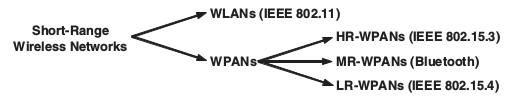
\includegraphics[scale=0.5]{./img/img_0__2_1}}
\\
\par 
Sieci typu WPAN możemy podzielić na 3 grupy: \\
\tab Sieci HR (high-rate) o wysokiej przepustowości danych, MR (medium-rate) sieci o umiarkowanej przepustowości oraz LR (low-rate) sieci o niskiej przepustowości. \\
\tab Przykładem sieci o wysokiej przepustowości może być siec służąca do streamingu w czasie rzeczywistym z kamery do HD-TV (jest to typowe zastosowanie standardu HR-WPAN IEEE 802.15.3), taki transfer sięga do prawie 60Mbs. Typowym reprezentantem sieci MR są rozwiązania oparte o Bluetooth z transferem sięgającym do 3Mbps który może służyć np. do wysokiej jakości transmisji głosowej. W skład ostatniej grupy LR wchodzi protokół ZigBee z maxymalną prędkością transferu sięgającą 250Kbps. \\


\clearpage

	\subsection{Rodzina standardów komunikacyjnych IEEE 802.15 :} 

\par IEEE 802.15 jest nazwą roboczej grupy standardów opracowanych przez "Institute of Electrical and Electronics Engineers" dotyczących dobrych praktyk oraz budowy aplikacji typu bezprzewodowa komunikacja radiowa na nielicencjonowanym paśmie częstotliwości którym w większości miejsc na świecie jest 2.4GHz. 
Standardów wchodzących w skład IEEE 802.15 jest siedem grup i wszystkie one dotyczą sieci bezprzewodowych typu WPAN (wireless personal area network).
WPAN jest to standard sieci bezprzewodowych zazwyczaj o niewielkim zasięgu służące do prostej komunikacji między urządzeniami. 
\par W sieciach tego typu dochodzi do komunikacji między dwoma lub większą ilością urządzeń i najczęściej istnieje podział na urządzenia podrzędne i nadrzędne.
Ze względu na budowę WPAN są najczęściej opisywane za pomocą modelu matematycznego jakim jest graf, z tego powodu urządzenia wewnątrz sieci są również nazywane węzłami sieci a połączenia między członkami sieci krawędziami.
\par WPAN mają wiele możliwości konfiguracji ze względu na wzajemne położenie lub funkcje urządzeń należących do sieci i jest nazywana potocznie architekturą sieci i określa ona zarówno wzajemne zależności funkcjonalne jak i fizyczne połorzenie węzłów sieci. 
Struktury wzajemnych połączeń tworzące architekturę mogą być stałe lub tworzone na bierząco dla określonej tymczasowej potrzeby. Dzięki temu sieci mają możliwość zmiany struktury sieci w ciągu kilki sekund.
Konkretnymi technologiami umożliwiającymi tworzenie sieci WPAN są Bluetooth, ZigBee, Z-Wave, Wireless USB, Ultra Wideband, IrDA, HomeRF/INSTEON i inne.
\\
\\
{\centering 
 Grupy standardów wchodzące w skład IEEE 802.15:
}
\\
\par - Group 1. WPAN/Bluetooth : najbardziej znana grupa bazująca na technologii Bluetooth definiuje warstwę fizyczną (PHY) oraz warstwę kontroli dostępu (MAC) Rozwiązania te powstały z myślą o przenośnych i mobilnych urządzeniach. Standard 802.15.1 ostatnio był aktualizowany w 2002 i 2005 roku.
\\
\par- Group 2. Standard IEEE 802.15.2 z 2003 roku dotyczy zalecanych praktyk dla technologii informatycznych w lokalnych i miejskich sieciach oraz współistnienia bezprzewodowych sieci i innymi urządzeniami bezprzewodowymi pracujących na nielicencjonowanym paśmie częstotliwości.
\\
\par- Group 3. High Rate WPAN : standard IEEE 802.15.3-2003 dotyczy dobrych praktyk i zaleceń odnośnie warstw fizycznej (PHY) oraz dostępu do medium (MAC) dla sieci z wysokimi prędkościami transferu tj. 11-55 Mbit/s. Grupa ta powstała z myślą o urządzeniach HDTV, "video on demand" czy "real time streaming" w których duże ilości danych (np. film) są transmitowane bezprzewodowo do odbiornika (np FullHD TV).
\\
\par- Group 4. Low Rate WPAN : standard traktujący o sieciach o niskiej szybkości transferu danych ale bardzo wysokiej energo-oszczędności głównie dla urządzeń o zasilaniu bateryjnym. 802.15.4 definiuje warstwę fizyczną (PHY) oraz warstwę łącza danych (data-link) czyli warstwy pierwzą i drugą modelu OSI. Pierwsza wersja standardu zostałą wydana w 2003 roku i obejmowała również wiele standaryzowanych oraz przemysłowych architektur sieci dla konkretnych protokołów korzystających z tego standardu takich jak:  ZigBee, 6LoWPAN, WirelessHART.
802.15.4 posiada również kilka rewizji (od a do g) większość z nich (a-e)była sporządzona w celu implementacji warstwy fizycznej na innych częstotliwościach niż bazowe 2.4GHz. Konieczność ta pojawiła się głównie ze względu na specyficzne przepisy w krajach takich jak Japonia, Chiny czy Korea.
\\
\par- Group 5. Mesh Networking : standard dostarczający architekturalne praktyki oraz zalecenia dla sieci WPAN w których skład wchodziły współpracujące ze sobą i zintegrowane High-Rate (IEEE 802.15.3) i Low-Rate WPAN (IEEE 802.15.4). 
\\
\par- Group 6. Body Area Networks : standard powstały w roku 2011 o nazwie BAN - Body Area Network. Są to sieci które cechują się wysoka energooszczędnością, krótkim zasięgiem działania o zastosowaniu na/w/wokół ludzkiego ciała (oraz nie tylko ludzkiego) które mają służyć do różnych zastosowań, w tym elektroniki medycznej, konsumenckiej i tej z branży osobistej rozrywki.
\\
\par- Group 7. Visible light communication : Grupa standardów powstałą w 2011 roku, IEEE 802.15.7 dotyczy implementacji warstw PHY i MAC dla komunikacji za pomocą światła widzialnego


\clearpage 
	%Bluetooth
	\subsubsection{Wprowadzenie do standardu 802.15.1 Bluetooth}

\par
\tab Standard Bluetooth jak wszystkie z rodziny IEEE.802.15 działa na częstotliwości 2.4 GHz. Wywodzi się on ze standardu 802.15.1 ale z czasem powstała specjalna grupa zajmująca się jedynie technologią Bluetooth i sam standard 802.15.1 przestał być rozwijany kosztem samego protokołu Bluetooth. Obecnie standard ten został wypuszczony w kilku wersjach: 1.0, 1.1, 1.2, 2.0,2.1, 3.0, 4.0, 4.1\\
Widmo sygnału rozciąga się od 2400 do 2483.5 MHz i zawiera w sobie 79 kanałów transmisyjnych każdy o częstotliwości 1MHz. (Standard 4.0 korzysta z 40 kanałów o szerokości 2MHz). Początkowo korzystał on jedynie z Modulacji GFSK (Gaussian frequency-shift keying) ale z czasem zaczęto stosować (wersje 2.0+) DQPSK  (Differential Quaternary Phase Shift Keying) i 8DPSK. \\

\par W przeciwieństwie do początkowych wersji standardu np. 1.0-2.0 która w zastosowaniu miałą być jedynie zamiennikiem dla przewodowego portu szeregowego, standard Bluetooth 4.0+ wprowadza bardzo wiele profilów dedykowanych do wielu różych zastosowań w tym do przesyłania muzyki czy danych a więc takich zastosowań w których przesyłane są duże bloki danych. \\
\par W bezprzewodowych sieciach sensorycznych, bardzo rzadko mamy doczynienia z dużymi transferami danych, ponieważ wiążą się one z dużym zurzyciem energii elektrycznej którego minimalizacja jest jednym z obecnych podstaw w projektowaniu sieci WSN. Twórcy standardu Bluetooth mając to na uwadze w wersji 4.0 dodali również profil Bluetooth Low Energy (nazywany również Bluetooth Smart), ma on za zadanie zapewnienie wolniejszego transferu danych z zachowaniem energooszczędności. \\
\par Sam Bluetooth jednak jest szybkim protokołem transmisyjnym i w celu implementacji wersji protokołu energooszczędnej, musiał zostać on gruntownie przerobiony w efekcie czego powstał Bluetooth smart, który z samym standardem 4.0 ma niewiele wspólnego, natomiast twórcy Bluetooth mogą się pochwalić rozwiązaniem które jest energooszczędne i stanowi część zbioru profili Bluetooth 4.0. \\
Z powodu różnic w budowie, które zostaną opisane w dalszej części pracy, występuje również różnica w użytkowaniu a mianowicie taka, że: urządzenie wyposażone w sam profil Bluetooth LE nie jest w stanie nawiązać komunikacji w urządzenie z bluetooth 4.0 (i niższym) które nie implementuje (najczęściej sprzętowo) standardu LE. Myśląc o Bluetooth należy rozróżniać że BLE i Bluetooth 4.0 mimo nazwy są fizycznie różniącymi się protokołami nie zawsze umożliwiającymi wzajemną transmisję. \\
Ponieważ w dalszej części pracy skupimy się na profilu Bluetooth Low Energy ze względu na możliwości wykorzystania w bezprzewodowych sieciach sensorycznych, niniejszy rozdział w skrócie przedstawia budowę protokołu Bluetooth w celu późniejszego porównania go do BLE. \\

\par 
\tab \textbf{Odkrywanie Urządzeń} \\
Tak jak wszystkie bezprzewodowe protokoły Bluetooth ma możliwość decydowania o nawiązaniu konkretnego połączenia z innym widocznym urządzeniem. Kanały Bluetooth dzielą się na tzw. \textit{piconet} oraz kanały rozgłośnieniowe. Aby urządzenie stało się widoczne musi ogłosić swoją obecność wysyłając pakiet zawierający ich adres. Kiedy urządzenie nawiąże połączenie dołącza do \textit{piconet-u} w ramach którego prowadzi połączenie natomiast ma również możliwość dalej rozgłaszać swoją obecność w sieci (co w przypadku BLE jest nie możliwe) \\

\par 
\tab \textbf{Architektura protokołu} \\
Bluetooth może być ogólnie podzielony na dwie części: Kontroler Bluetooth oraz Host. \\
Protokołem transportowym jest analogiczny do TCP - RFCOMM który jest używany do emulowania portu szeregowego, wysyłania tzw. AT command (standardowy protokół wykorzystywany w urządzeniach typu serial-port). \\
Ponieważ standard bluetooth definiuje architekturę host-kontroler najniższą warstwą łączącą kontroler i host-a jest tzw.  \textit{Host-Controller-Interface} w której odbywa się nawiązywanie połączenia czy zakończenie transmisji. \\
Oprócz HCI występuje jeszcze warstwa LMP \textit{Link Manager Protocol} w której znajduje się stos protokołu oraz odbywają niskopoziomowe kwestie związane z kryptografią autentykacją oraz parowaniem \\
Najniższą warstwą związaną bezpośrednio z transmisją jest \textit{Baseband controller} odpowiedzialny za fizyczną transmisję radiową oraz obsługę radia.

\clearpage 
	\subsubsection{Standard 802.15.4}

\par
\tab \textbf{Definicja protokołu} \\
Standard IEEE 802.15.4 jest standardem dla warstwy fizycznej oraz dostępu do medium komunikacyjnego dla sieci LR-WPAN (low rate wireless personal area networks). Skupia się on na podstawowych najniższych warstwach komunikacji. Architektura protokołu bazuje na modelu OSI, jednakże tylko najniższe warstwy są ściśle ustandaryzowane mechanizmami takimi jak np. CSMA. Do interakcji z górnymi warstwami można użyć zalecanej normy IEEE 802.2 który określa logiczną podwarstwę sterowania dostępem do warstw wyższych z warstwy MAC poprzez warstwy pośrednie.

\par
\tab \textbf{Specyfikacja widmowa} \\
Istnieją trzy pasma częstotliwości przewidziane dla standardu IEEE 802.15.4 które zostały zdefiniowane ostatnio w roku 2006
\begin{enumerate}
	\item 868-868.6 MHZ (868MHz band)
	\item 902–928  MHz (915 MHz band)
	\item 2400–2483.5 MHz (2.4 GHz band)
\end{enumerate} 

Pasmo 868 MHz jest wykorzystywane w Europie w wielu aplikacjach bezprzewodowych krótkiego zasięgu, 915 MHz natomiast jest używane w Północnej Ameryce oraz Australii. Pasmo 2.4 GHz jest z koleji powszechnie wykorzystywane na całym świecie. \\

\par
\tab \textbf{Charakterystyka częstotliwościowa} \\
W sieciach IEEE 802.15.4 występuje kila dopuszczalnych modulacji częstotliwościowych: BPSK, ASK czy O-QPSK. Bezpośrednio metoda modulacji przenosi się na dopuszczalne prędkości transmisji danych i tak dla modulacji BPSK będzie to 40Kb/s, ASK 250 Kb/s a dla O-QPSK 250 Kb/s. \\
Szczegółowa charakterystuka znajduje się w tabeli poniżej: \\

\mbox{}\\
\begin{tabular}{ |p{2cm}||p{1.5cm}|p{1.5cm}|p{1.8cm}|p{1.8cm}|p{1.8cm}|p{3cm}|  }
 \hline
 Częstot. (MHz) & Chann nr. & Modulacja & Chip Rate (Kchip/s) & Bit Rate (Kb/s) & Symbol Rate (Ksymb/s) & Modulacja Widma \\
 \hline
868–868.6 & 1 & BPSK & 300 & 20 & 20 & Binary DSSS \\
 \hline
902–928 & 10 & BPSK & 600 & 40 & 40 & Binary DSSS \\
 \hline
868–868.6 & 1 & ASK & 400 & 250 & 12.5 & 20-bit PSSS \\
 \hline
902–928 & 10 & ASK & 1600 & 250 & 50 & 5-bit PSSS \\
 \hline
868–868.6 & 1 & O-QPSK & 400 & 100 & 25 & 16-array orthogonal \\
 \hline
902–928 & 10 & O-QPSK & 1000 & 250 & 62.5 & 16-array orthogonal \\
 \hline
2400–2483.5 & 16 & O-QPSK & 2000 & 250 & 62.5 & 16-array orthogonal \\

 \hline
\end{tabular}
\mbox{}\\

\par
\tab \textbf{Budowa standardu} \\
Sam standard IEEE 802.15.4 definiuje dwie warstwy: Warstwę fizyczną połączenia (PHY) oraz warstwę sieciowią (MAC). W warstwie MAC główne funkcjonalności sieci  opierają się na nadzorowaniu oraz nawiązywaniu połączenia, zarządzaniu transmisją oraz adresacją samego urządzenia. Natomiast w warstwie PHY następuje zamiana pakietów na strumień bitów, modulacja oraz bezpośrednia transmisja radiowa. \\

\par
\tab \textbf{Charakterystyka urządzeń w sieci 802.15.4} \\
Standard IEE 802.15.4 definiuje trzy główne role urządzeń w sieciach WPAN ze względu na funkcję pełnioną w całej sieci PAN.
\begin{enumerate}
	\item PAN Coordinator (FFD)
	\item Coordinator (FFD)
	\item Device (RFD or FFD)
\end{enumerate}  

\clearpage
	\subsubsection{Zależność między standardem IEEE 802.15.4 a Zigbee }

\tab Podstawowym podejściem służącym do ustabilizowania złożonych rozwiązań technologicznych jest podział na autonomiczne moduły-warstwy. Podejście to jest szeroko stosowane w protokołach sieciowych gdzie spotykamy wielowarstwowe modele sieci z których każda warstwa jest odpowiedzialna za pewne z góry określone funkcję w sieci. Dane mogą być przesyłane z jednego poziomu do wyższej lub niższej warstwy.

\tab Protokół ZigBee bazuje na dobrze znanym modelu OSI (Open System Interconnect). Podział Zigbee na warstwy przynosi wiele korzyści, z których główną jest możliwość modyfikacji lub nawet zamiany całej warstwy w wyniku ewolucji technologicznej co w przypadku monolitycznych rozwiązań wiąże się z refaktoryzacją całego protokołu. \\

\par Historia Zigbee: \\ 

Nazwa ZigBee: stanowi nawiązanie do "tańca pszczół" czyli regularnych cyklicznych ruchów za pomocą których pszczoły informuują inne robotnice o wykonywanym zajęciu \\ 
\tab 	Historia powstania ZigBee sięga jeszcze ostatnich lat 20 wieku, kiedy to odbyło się wiele dyskusji w kręgach inżynierskich nad zastosowaniem komunikacji bezprzewodowej opartej na obecnych wtedy na rynku rozwiązań bazujących na WiFi lub bluetooth-u. Pierwszym kompletnym standardem który powstał w 2003 roku był IEEE 802.15.4 \\

\par \tab \textbf{Warstwowa budowa protokołu 802.15.4 i ZigBee} \\ 

\tab 	Jak wcześniej zostało powiedziane standard IEEE 802.15.4 jest standardem dla warstwy fizycznej oraz dostępu do medium komunikacyjnego, jego funkcjonalności kończą się na "bezpośrednim transferze pakietów, oraz zarządzaniu transmisją w sieci". Stanowi on bezpośrednią bazę na której można oprzeć bardziej rozbudowane protokoły komunikacyjne które oprócz prostego transferu wykorzystują w swoim działaniu inne mechanizmy takie jak ruting, broadcasting, uwierzytelnianie. \\
\\
Koncepcyjną budowę warstwową protokołu ZigBee przedstawia poniższy schemat: \\
\centerline{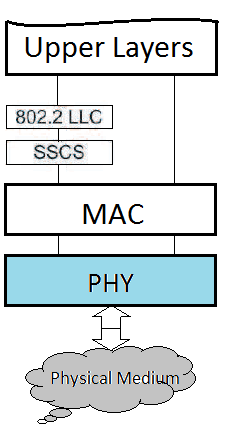
\includegraphics[scale=0.5]{./img/img_1__2_1_3}}
\\

\par \tab \textbf{802.15.4 Fizyczną i sieciową warstwa ZigBee:} \\ 
\tab 	ZigBee jest standardem komunikacji radiowej. W swoich założeniach zaleca komunikację na częśtotliwościach 2.4 GHz (stosowane na całym świecie) oraz ze względu na panujące prawo determinujące komumikację radiową: dodatkowe pasmo na częstotliwości 915 MHz dla Ameryki i Australii oraz 868 MHz dla Europy. \\
\tab 	Pasmo 2.4 GHz umożliwia transmisję o prędkości maksymalnej do 250Kbps oraz udostępnia 16 różnych kanałów transmisyjnych. 915 MHz (w rzeczywistości 902–928MHz) daje możliwość rozwinięcia prędkości 40Kbps i udostępnia 10 kanałów transmisyjnych, natomiast 868 MHz daje możliwość transmisji do 20Kbps i 1 kanał transmisyjny.\\
Standard ZigBee opierający się o normę 802.15.4 definiuje szeref mechanizmów zapewniających niezawodność transmisji danych. W warstwie fizycznej, dla częstotliwości 868/915 MHz jest wykorzystywane kodowanie "Binary Phase Shift Keying" czyli modulacji cyfrowej polegającej na kluczowaniu fazy, natomiast dla 2.4GHz transmisja wykorzystuje inną odmianę modulacji fazy O-QPSK. Są to proste szybkie metody modulacji które sprawdzają się dobrze w środowiskach o niskim stosunku SNR. \\

\par \tab \textbf{ Warstwa MAC i mechanizmy wchodzące w jej skład} \\ 
\tab 	CSMA jest mechanizmem definiowanym przez standard IEEEumożliwiającym urządzenią współdzielenie tego samego kanału transmisyjnego, zapobiegającemu występowaniu kolizji. Technika ta pochodzi z przed lat a jej mechanizm był wykorzystywany w sieciach Ethernetowych, dzięki czemu urządzenia nie potrzebowały się synchronizować między sobą. Metoda wielodostępu do tego samego kanału jest bardzo prosta i intuicyjna, opiera się na zasadzie "listen before you talk". Czyli każde urządzenie przed rozpoczęciem nadawania nasłuchuje na danym kanale i jeśli jest obecnie wolny nadaje wiadomość, w przeciwnym wypadku odczekuje okres czasu zależny od platformy i powtarza czynność dopóki kanał się nie zwolni, lub odczekiwany okres czasu przekroczy założony interwał i zgłosi błąd transmisji.\\
\tab 	Mechanizm potwierdzania/ponawiania transmisji służy w sytuacji kiedy wiadomość zostanie poprawnie nadana jednak odbiorca nie będzie w stanie jej dobrze odebrać (np w sytuacji kiedy nie zgadza się suma kontrolna, lub rozmiar ramki). Każde urządzenie w momencie odebrania wiadomości ma krótki czas w którym musi wysłać potwierdzenie odbioru nazywane dalej ACK. Jeśli nadawca nie dostanie zgłoszenia ACK, przyjmuje on że z jakiś powodów wiadomość nie dotarła do odbiorcy i ponownie wysyła tę samą ramkę danych, ponownie czekając na potwierdzenie od odbiorcy. Proces ten jest powtarzany dopóki odpowiedź ACK nie zostanie odebrane lub nadawca przekroczy zdefiniowany przez siebie czas i zgłosi niedosłanie wiadomości.\\	
\tab 	IEE 802.15.4 określa specyfikacje dotyczące PHY i sposobu adresowania za pomocą numerów MAC, dostarczając gotowe topologie dostosowane do systemów o różnym zastosowaniu poczynając od prostych architektór takich jak peer-to-peer czy star (gwiazda) a kończąc na takich jak mesh (nie skorelowane równoważne węzły) i cluster tree (architektura składająca się z połączonych drzew rozpiętych na blokach odbiorników). W zależności od architektury i zastosowania stosuje się systemy routingu które zaprojektowane głównie w celu zapewnienia ochrony energii spełniają również takie funkcje jak zapewnienie niskiej latencji dla transmitowanych danych, niezawodność transmisji oraz w ujęciu calościowym dla sieci odporność na uszkodzenia, niezawodność i elastyczność. \\

\par \tab \textbf{Komponenty wchodzące w skład sieci:}\\ 
\tab Sieci ZigBee zawierają wiele  komponentów składowych. Podstawą jest urządzenie z którym chcemy się komunikować. Może być nim każdy układ elektroniczny np: sensor, interfejs graficzny urządzenie wejścia/wyjścia. Urządzenie to może być nazwane mianem FFD (full-function device) lub RFD (reduced-function device). Aby sieć miała sens funkcjonalny musi zawierac conajmniej jedno urządzenie FFD które stanie się koordynatorem sieci (w literaturze PAN (personal network area) coordinator). Dzięki koordynatorowi informacje zebrane z sieci mogą być przesłane dalej lub przetwarzane na miejscu. \\
\tab		Urządzenie FFD może pracować w 3 trybach: jako PAN coordinator, coordinator lub zwykłe urządzenie, natomiast urządzenia typu RFD są przewidziane do prostych zastosowań nie wymagających wysyłania dużej ilości danych. Urządzenie FFD może prowadzić komunikację z jednym lub wieloma urządzeniami RFD jednocześnie natomiast RFD może prowadzić komunikację jedynie z 1 FFD.
\\		
\begin{center}
Topologie sieci zdefiniowane przez standard IEEE 802.15.4: \\
\end{center}
Ciekawą częścią standardu IEEE 802.15.4 która powrzechnie jest wykorzystywana w aplikacjach WPAN są określone możliwe topologie sieci, które wiążą się bezpośrednio z warstwą sieciową i tym w jaki sposób sieć jest zarządzana przez koordynatora sieci.
\par 
Star Topology (Topologia gwiazdy):\\ 
\tab 	W topologii gwiazdy komunikacja jest nawiązana pomiędzy urządzeniami należącymi do sieci oraz pojedyńczą centralną jednostką kontrolera PAN coordinator. W analizie sieci przyjmuje się że PAN może być zasilany sieciowo natomiast urządzenia stanowiące wierzchołki gwiazdy są zasilane bateryjnie. \\
\tab 	Konfiguracja sieci rozpoczyna się od aktywacji pierwszego urządzenia FFD które może zostać koordynatorem sieci. Urządzenia mogą wybrać czy dany FFD może zostać  PAN coordinator-em sieci. Każde uruchomienie sieci powoduje na nowo wybór koordynatora sieci lub jego identyfikacje i sprawdzenie czy nie należy on już do innej sieci. Dzięki temu sieci o topologii gwiaździstej mogą pracować niezależnie od reszty otoczenia sieciowego.\\

\par 
Topologia Peer-to-peer:\\ 
\tab		W topologii peer-to-peer podobnie jak w topologii gwiazdy mamy do czynienia z jednym urządzeniem pełniącym funkcję PAN coordinator, natomiast w porównaniu do topologii gwiazdy urządzenia mają swobodę komunikacji i mogą wymieniać ramki danych z każdym innym a nie tylko z koordynatorem. Sieci peer-to-peer dzięki swobodzie w komunikacji mogą być typu ad-hoc, self-organizing lub self-healing. Dzięki wielostopniowemu rutingowi sieci te zyskuja bardzo dużo na niezawodności.\\
\par
Topologia Cluster-tree:\\ 
\tab		Sieci typu Cluster-tree są specjalnym przypadkiem w którym mamy doczynienia z kilkoma sieciamy typu peer-to-peer których koordynatorzy porozumiewają się między sobą na zewnątrz podsieci. Każda z podsieci staje się wtedy częścią nowego dużego drzewa. Po uruchomieniu sieci ze wszystkich koordynatorów tworzących podsieci jest wyłaniany jeden główny PAN coordinator, natomiast wszyscy inni lokalni koordynatorzy mogą swobodnie w swoich sieciach prowadzić takie operacje jak synchronizacja transmisja czy renegocjacje między urządzeniami. Po wyborze PAN coordinatora staje się on główną częścią klastra z CID (cluster ID) równym zero, następnie rozsyła on i przydziela identyfikatory swoim sąsiadą. Jeśli zdecyduja się oni dołączyć do sieci rozdają kolejne wolne CID-y swoim sąsiadą, dzięki czemu w sieciach lokalnych może następować komunikacja jak to miało miejsce w sieciach peer-to-peer natomiast jednocześnie wszystkie urządzenia są dostępną dla siebie częścią klastra.\\

\clearpage 
	\subsection{Budowa protokołu ZigBee}

ZIGBEE layers! opisac

\clearpage
	\subsection{Budowa protokołu Bluetooth Low Energy}

\clearpage
	\subsection{Bezprzewodowe sieci sensoryczne}

\subsubsection{Wprowadzenie}

\par 
\tab 	Pojęcie bezprzewodowych sieci sensorycznych jest używane w odniesieniu do autonomicznych rozproszonych sensorów które oprócz podstawowej funkcji jaką jest zbieranie danych z otoczenia lub układu pomiarowego również są w stanie komunikować się między sobą, jednakże komunikacja ta jest wykorzystywana głównie do transportu pakietów do koordynatora sieci lub z koordynatora do urządzeń końcowych czyli sensorów.
W literaturze angielskiej sieci te są nazwane \textit{Wireless sensor network} w skrócie \textbf{WSN} i stanowią one podzbiór sieci wchodzących w skład rodziny sieci typu \textit{Wireless personal area networks} czyli \textbf{WPANs}.
\\
Nowoczesne sieci WSN są projektowane na wzór aplikacji wojskowych takich jak tzn: \textit{battlefield surveillance} czyli sieci które są samoorganizacyjne i odporne na awarie czy zniszczenia.
Przeznaczenie sieci sensorycznych jest bardzo zróżnicowane poczynając od prostych aplikacji w których jednostka centralna komunikuje się z kilkoma sensorami a kończąc na rozległych sieciach z wieloma podsieciami. Są one stosowane we wszystkich dziedzinach przemysłu poczynając od aplikacji konsumenckich takich jak inteligentne domy a kończąc na rozwiązaniach specjalistycznych takich jak przemysł militarny, urządzenia medyczne czy przemysł kosmiczny.
\\
\par Podstawową autonomiczną jednostką która wchodzi w skład sieci WSN jest węzeł. Każdy z węzłów jest połączony do conajmniej jednego węzła w sieci. Sieć może składać się od kilku do tysięcy komunikujących się ze sobą węzłów. Sieci sensoryczne z góry nie narzucają technologii za pomocą której węzły sieci komunikują się ze sobą, WSN jest określeniem bardziej samego zastosowania sieci niż jej konkretnej implementacji sprzętowej czy programowej, jednak zwykło się określać nazwą \textit{Wireless Sensor network} sieci posiadając następujące cechy charakterystyczne: \\
\\
\begin{itemize}
  \item Wymaganie energooszczędności od autonomicznych węzłów sieci
  \item Umiejętność radzenia sobie z awariami węzłów
  \item Możliwość przemieszczania się, znikania z sieci węzłów bez szkodliwych skutków dla całej sieci
  \item Możliwość wzajemnej współpracy heterogenicznych węzłów
  \item Skalowalność
  \item Odporność na trudne warunki środowiskowe
  \item Transparentność między podsieciami
  \item Cross-level Design.
\end{itemize}
\par Cross-Level Design: \\
Pojęcie Cross-Level-Design jest to akademicka definicja stosowana w odniesieniu do sieci wielowarstwowych które to rozwiązuje problem wynikający z limitów pewnych warstw sieci (najczęściej limitów warstwy fizycznej) poprzez oddelegowanie problemu do wyższej warstwy sieci.
Przykładem może być typowy problem efektywnej transmisji w obciążonych wielowęzłowych sieciach heterogenicznych. Ponieważ najniższa warstwa jaką jest PHY posiada pewne fizyczne limity które są opisane w standardzie 802.15 następuje sprzężenie zwrotne między warstwą fizyczną i wyższymi warstwami. Mechanizmami które powstały specjalnie ze względu na CLD są np: samoorganizacja sieci, automatyczna zmiana kanałów nadawania czy algorytmy routingu.\\
Podejsciem odwrotnym do \textit{Cross-layer} jest tzw. \textit{layered module} czyli klasyczne podejście polegające na rozbudowywaniu warstwy w taki sposób aby problemy danej warstwy były rozwiązywane na jej poziomie.
\\

\subsubsection{Komponenty sieci WSN :} 

\par Węzeł sieci (\textit{Node}) : \\
\tab Węzłem sieci jest nazywany zbiór modułów wchodzących w skład jednego czujnika. Typowo sensor składa się z jednostki kontrolnej oraz jednostki transmisyjnej. Najbardziej typowym designem jest połączenie mikrokontrolera (jednostki kontrolnej) z układem nadawczym radiowym oraz blokiem odpowiadającym za zarządzanie poborem mocy. Projektując sieci najczęściej dąży się do tego aby węzły sieci były jak najbardziej proste i nie skomplikowane. Zarządzanie mocą realizowane najczęściej za pomocą zasilania bateryjnego i układów oszczędzania energii, jest stosowane w celu zapewnienia sieci cechy mobilności i reorganizacji węzłów.
\\
\par Koordynator sieci : \\
\tab
\\
\par Koordynator sieci : \\
\tab



\clearpage
	\subsection{Omówienie zagadnień bezpieczeństwa siecy typu Wireless Sensors Network}

\subsubsection{Bezpieczeństwo i poufność danych w sieciach bezprzewodowych}

\par
\tab W dziedzinie jaką jest transmisja informacji u fundamentów stoi zdolność do właściwego przekazu informacji tak aby obie strony uczestniczące w wymianie informacji były w stanie się na wzajem zrozumieć. Kolejną z ważnych cech protokołu komunikacyjnego jest zdolność do zapewnienia bezpieczeństwa przesyłanych informacji. \\
W klasycznych przewodowych protokołach komunikacyjnych bezpieczeństwo było zapewniane za pomocą fizycznych metod takich jak brak dostępu do medium transmisyjnego jakim był kabel prze zabiegi takie jak izolacja, ekranowanie czy wytłumianie sygnału elektrycznego poza przewodem, dzięki temu już na początku w sieci znajdują się tylko zaufane znane urządzenia którym na ten dostęp przyzwolono co znacząco upraszcza kwestię związane z bezpieczeństwem informacji. \\
\tab W protokołach bezprzewodowych kwestię związane z bezpieczeństwem są dużo bardziej skomplikowane z oczywistego powodu jakim jest natura działania protokołu opierająca się na zjawisku propagacji fal elektromagnetycznych w przestrzeni. W związku z tym każdy wyposażony w odbiornik jest w stanie odebrać wysyłane wewnątrz sieci pakiety. W sieciach wielokrotnie złożonych jakimi są np. WSN sytuacja często jest jeszcze bardziej skomplikowana ponieważ pakiety wędrują nie tylko między dwoma węzłami ale mogą one być transmitowane między dziesiątkami lub setkami heterogenicznych węzłów i/czy sieci.  
W większości nowoczesnych sieci bezprzewodowych koniecznym wymogiem co do bezpieczeństwa są książkowe cechy: poufność, integralność, uwierzytelnianie, dostępność, autoryzacja i niezaprzeczalności.  \\
Z uwagi na różnice funkcjonalne i architekturalne trudno jest omówić jednocześnie bezpieczeństwo sieci WPAN z tego powodu w tym rozdziale szczegółowo zostaną omówione sposoby w jaki najpopularniejsze obecnie sieci \textit{WPAN} czyli ZigBee i \textit{Bluetooth smart} zapewniają i implementują mechanizmy bezpieczeństwa danych. \\

\subsubsection{Mechanizmy Bezpieczeństwa w sieciach ZigBee}

\par Wprowadzenie: \\
\tab W prostych aplikacjach typu sensor-odbiornik względy bezpieczeństwa często mogą być pomijane, natomiast w każdym odpowiedzialnym zastosowaniu względy bezpiecznego transmitowania danych muszą być brane pod uwagę. \\
Zigbee ze względu na ilość potencjalnych wykorzystań w przemyśle oczywiście implementuje mechanizmy kryptograficzne.

\paragraph{Kryptografia symetryczna w sieciach ZigBee} 

\par Standard ZigBee był projektowany z myślą o prostych mobilnych sensorach które mogłyby być swobodnie dołączane oraz odłączane z sieci. Ze względu na prostotę sensorów oraz ich energooszczędność (a konkretniej sposb zasilania ktory jest najczesciej bateryjny) najczęściej jednostki centralne czujników są realizowane za pomocą mikrokontrolerów o ograniczonych zdolnościach obliczeniowych. Z tego względu podstawową metodą szyfrowania danych wspieraną przez protokół ZigBee jest kryptografia symetryczna realizowana przez algorytm szyfrujący AES (\textit{Advanced Encryption Standard})
Na poniższym schemacie jest pokazana ogólna koncepcja szyfrowania danych w protokole ZigBee. \\
\centerline{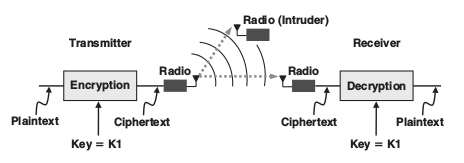
\includegraphics[scale=0.5]{./img/img_zigbee_aes}}

Niezaszyfrowana wiadomość jest nazywana \textit{plaintext} czyli tekstem jawnym natomiast zaszyfrowana nosi w literaturze obcojęzycznej nazwę \textit{ciphertext} czyli kryptogram. Algorytmy szyfrujące do jakich zalicza się AES są typowo algorytmami blokowymi, ponieważ tekst jawny dzieli się na bloki które następnie są szyfrowane, również przy odszyfrowywaniu kryptogram jest dzielony na bloki które są odszyfrowywane za pomocą tajnego klucza. ZigBee używa 128 bitowych bloków szyfrujących/deszyfrujących. \\
AES jest algorymtem symetrycznym stąd szyfrowanie i deszyfrowanie jest realizowane za pomocą tego samego klucza który jest z założenia tajny i jedynie porozumiewające się strony mają do niego dostęp. Klucz szyfrujący jest w postaci binarnej i jest umieszczany w odpowiednich urządzeniach za pomocą różnych technik o których często decyduje producent układów lub konstruktor rozwiązania wykorzystującego WSN.
Zigbee wspiera klucze szyfrujące AES wielkości 128, 196 i 256bitów, oraz implementuje metody rozdzielania i utrzymywania tych kluczy w sieci. Pomimo faktu, że sieci standard dopuszcza jedynie możliwość symetrycznej kryptografii podczas transmisji są wykorzystywane w praktyce dwa symetryczne klucze: \textit{linked key} oraz \textit{network key}. \\
\textit{Linked key} jest kluczem dzielonym jedynie między dwoma węzłami i jest on wykorzystywany w pojedyńczej komunikacji.\\
\textit{Network key} natomiast jest współdzielony przez wszystkie urządzenia mające dostęp do sieci i jest wykorzystywany do samego procesu dołączenia do sieci, oraz komunikacji jeden do wielu (\textit{broadcasting}). \\ 
Sieć implementująca szyfrowanie wiadomości musi również posiadać urządzenie o specjalnym przeznaczeniu tzn. cenfrum zaufania (\textit{trust center}). Może nim być koordynator sieci ale również każde inne urządzenie warunek jest taki że jedna sieć ma jedno i tylko jedno centrum zaufania które służy do dystrybucji kluczy, i jego adres jest ustalany przez koordynatora sieci.

\paragraph{Trust center i mechanizmy zarządzania kluczami} 

\par W poprzednim paragrafie zostało wspomniane o dwóch kluczach występujących w sieciach ZigBee a mianowicie o dynamicznie przyznawanym \textit{Linked Key} oraz permanentnym przypisanym do sieci \textit{Network Key}. Istnieją trzy metody przypisywania klucza do urządzenia: preinstalacja (\textit{preinstallation}), transportowanie klucza (\textit{key transport}) oraz ustalenie klucza (\textit{key establishment}). \\
Preinstalacja polega na wbudowaniu klucza podczas procesu wytwarzania. Metoda ta często jest potocznie nazywana hardcodowaniem klucza i może odbywać się na różne sposoby np. generowanie klucza podczas procesu programowania urządzenia i zapisywanie go w pamięci nieulotnej, jak i również na umieszczaniu go w specjalnej sekcji na etapie samego wytwarzania krzemowego układu. Korzystając z takiego rozwiązania urządzenia przyłączające się do sieci nie potrzebują odpytywać \textit{trust center} o klucz sieciowy ponieważ już nim dysponują. W wielu aplikacjach preinstalacja jest najbardziej bezpieczną metodą rozprowadzania tajnego klucza sieciowego ponieważ jest on przekazywany jedynie na etapie produkcji który z założenia jest bezpieczny.\\
Metoda transportowania klucza polega na procesie odpytywania poprzez urządzenie przyłączone do sieci \textit{trustcenter} o klucz sieciowy. Całość zapytania odbywa się w warstwie APS, w której \textit{trustcenter} decyduje czy wysłać urządzeniu klucz sieciowy czy też nie. powyższasesja odbywa się za pomocą nieszyfrowanego połączenia, co oczywiście stanowi istotną lukę bezpieczeństwa uniemożliwiającą stosowanie tej metody w wielu krytycznych zastosowaniach. Rozwiązaniem tego problemu jest stosowanie tzw. \textit{key-transport key}. KTK używa dodatkowego klucza który jest wykorzystany do transmisji tajnego klucza. \\
Trzecią z metod jaką jest przypisywanie poprzez ustalenia klucza polega na stworzeniu losowego klucza między dwoma komunikującymi się ze sobą urządzeniami omijając nieszyfrowane bezprzewodowe kanały komunikacyjne. W sieciach WSN bazujących na protokole ZigBee protokół ustalania klucza korzysta z symetrycznego protokołu ustalania klucza (





	
	%Part 3 implementacja systemu WSN/RT
	\section{Implementacja Systemu WSN/RT}

\newtheorem{rt_book_def}{Definicja "książkowa"}[section]
\newtheorem{rt_practic_def}{Definicja "praktyczna"}[section]
\subsection{Systemy Real Time}
\subsubsection{Podstawowe pojęcia}

\par
\tab Definicja pojęcia bezpieczeństwa systemów czasu rzeczywistego odbiega znacznie od  bezpieczeństwa rozumianego w kontekście klasycznych systemów operacyjnych lub tego z którym spotykamy się podczas problemów związanych z IT-Security. \\
Czym w takim razie jest Real-Time?

\begin{rt_book_def}
Poprawność wykonania operacji
zależy nie tylko od tego, czy
wykonała się bez błędów i zwróciła
poprawny rezultat, ale także od czasu
(górnego ograniczenia) w jakim
operacja się zakończyła.
\end{rt_book_def}

Oznacza to, że o funkcji/operacji możemy powiedzieć że jest czasu rzeczywistego jeśli oprócz tego że wykonany wynik jest "bezbłędny" to również czas wykonania jest z góry określony przez pewne maximum. 

\begin{rt_practic_def}
System RT, to taki, w którym da się
udowodnić, że każda wymagana
operacja zakończy się w określonym
czasie.
\end{rt_practic_def}

W idealnym przypadku jest to dowód matematyczny. Niestety
przy złożoności współczesnych systemów w większości przypadków jest to niewykonalne,
a nawet jeżeli, to istnieje ryzyko popełnienia błędu podczas
dowodzenia. \\
\tab W praktyce stosuje się zestaw testów. System, który przejdzie
takie testy określne w specyfikacji lub powstające podczas jego
tworzenia, jest określany jako system czasu rzeczywistego. 
Testy takie przeprowadza się mierząc czas odpowiedzi na badany sygnał przy otaczających
niekorzystnych dla systemu warunkach, jeśli czas odpowiedzi (deadline) jest deterministyczny to wtedy możemy sądzić że system przeszedł testy pomyślnie.\\

\textbf{Deadline} systemu czasu rzeczywistego nazywamy "Punkt w czasie, w którym dana akcja ma nastąpić (np. reakcja na zmianę stanu wejścia)."

Ze względu na podział systemów czasu rzeczywistego na podgrupy (Hard-RT, Soft-RT) rozróżniamy różnice w pojmowaniu Deadline. \\

\textbf{Hard Real-Time} - operacja zawsze \textbf{musi} zakończyć się w
określonym czasie. Wynik operacji zakończonej później - nie nadaje
się do wykorzystania (awaria już nastąpiła). \\

\textbf{Soft Real-Time} - okazjonalnie operacja \textbf{może} zakończyć się po
ustalonym czasie (błąd nie jest krytyczny dla operacji). \\

Czas pomiędzy momentem w którym akcja miała wystąpić, a momentem w którym w rzeczywistości wystąpiła nazywamy \textbf{opóźnieniem} systemu-RT (Latency). 
W idealnym przypadku (taki system nie istnieje) - opóźnienia
byłyby zerowe. W rzeczywistości komputer potrzebuje pewnego czasu na
ustabilizowanie i przetworzenie sygnałów ze sprzętu,
oprogramowanie wprowadza własne opóźnienia itp. \\ \\
\textbf{Jitter}: wariancja opóźnienia (poprzedniej wartości). Z powodu, że czas pomiędzy wystąpieniem przerwania (zgłoszeniem przez sprzęt) a uruchomieniem procedury jego obsługi nie jest stały mamy doczynienia z wariancją czasów opóźnień, jej zmienność jest równie groźna jak duże opóźnienie (na
przykład uniemożliwia wykorzystanie systemu do akwizycji danych). \\ \\

\textbf{Predictability} Przewidywalność: oznacza wiedzę na temat tego ile czasu zajmie operacja (na
przykład procedura obsługi przerwania).
Teoria algorytmów zajmuje się określaniem złożoności
obliczeniowej poszczególnych metod. W szczególności aby system
był przewidywalny, konieczne jest używanie algorytmów
działających w stałym czasie (niezależnym od ilości danych). \\ 

\textbf{Worst Case} Najgorszy przypadek : ze względu na zmienność rzeczywistych systemów (nie da się zbudować systemu idealnego), głównym polem naszych
zainteresowań pozostaje „najgorszy możliwy przypadek”.
System będzie działał w sposób przewidywalny jeżeli będziemy
znać jego opóźnienie w najgorszym możliwym przypadku.
\clearpage

\subsubsection{Sygnały wejścia/wyjścia}

\par
\tab W ogólnym przypadku systemy cyfrowe lub mikrokontrolerowe oddziaływują ze światem zewnętrznym za pomocą portów wejścia/wyjścia. Porty te mogą być połączone do zewnętrznych czujników i stanowić, magistrale cyfrowe za pomocą których jednostka centralna (mikroprocesor, układ fpga) otrzymuje sygnały pochodzące ze świata zewnętrznego które są zbierane przez czujniki, czy linie za pomocą których mikrokontroler zbiera i analizuje sygnał elektryczny w postaci napięciowej i samodzielnie konwertuje sygnał do postaci cyfrowej. \\
\tab O ile możliwości dostarczania informacji jest bardzo wiele ponieważ istnieje niezliczona ilość czujników które można podłączyć do systemu cyfrowego, istnieją dwa główne sposoby reakcji systemu mikroprocesorowego na zmianę sygnału wejściowego nie zależnie czy odczyt z portu wejścia jest informacją cyfrową czy analogową. Ponieważ każda informacja i tak finalnie jest przetwarzana do postaci cyfrowej rozróżniamy: \textit{wejścia próbkowane ciągle} oraz \textit{wejścia sterowane przerwaniami}.

\par
\tab Wejścia ciągle próbkowane (continuous sampling port detection). W najprostrzej wersji metodę tę można przedstawić z programistycznego punktu widzenia jako nieskończoną pętle w której procesor odczytuje co okreśnoną jednostkę czasu synchronicznie stan komórki pamięci w której jest przechowywany odczyt z zewnętrznego czujnika, i porównuje tę wartość z jakąś inną wartością i w zależności od wyniku porównania następuje określona akcja. \\ 

\centerline{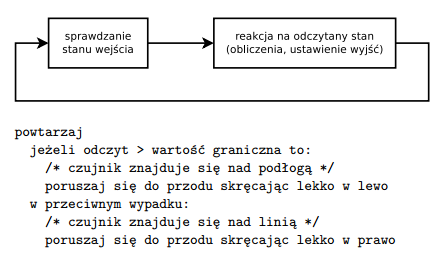
\includegraphics[scale=0.75]{./img/target_system/continius_sampling.png}}
\centerline{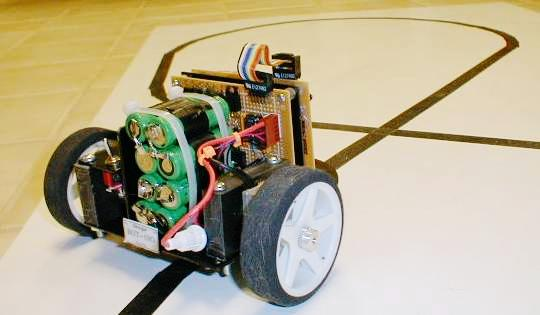
\includegraphics[scale=0.35]{./img/target_system/line_following_robot.jpg}}

\par
\tab Wejścia sterowane przerwaniami są natomiast asynchronicznym sposobem reagowania na zdarzenie przychodzące z zewnątrz. System wykonuje program główny w oderwaniu od zdarzeń zewnętrznych do czasu nadejścia przerwania które wywłaszcza czas procesora na krótki okres podczas którego musi zostać obsłużone. Często takie przerwania są właśnie sygnałami czasu rzeczywistego które przychodzą nagle w odpowiedzi na jakieś zewnętrzne zdarzenie i muszą być jak najszybciej obsłużone. \\ 

\centerline{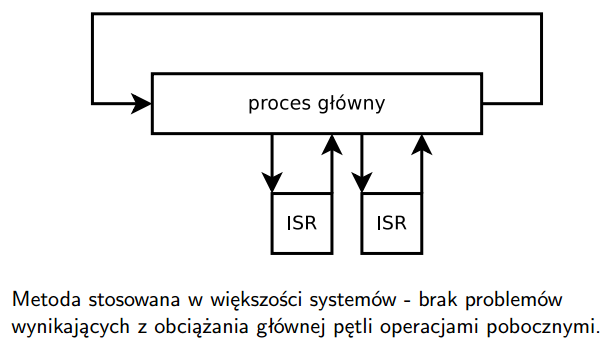
\includegraphics[scale=0.50]{./img/target_system/interrupt_driven_port.png}}

\par 
\tab Najprostrzym układem wzorcowym którym posłużymy się do opisu układu czasu rzeczywistego będzie prosty układ elektryczny zawierający przełącznik dwustanowy (wł/wył) oraz diodę LED. W momencie kiedy zewrzemy przełącznik (stan wł) dioda momentalnie się zapali ponieważ przez zwarty przełącznik zacznie płynąć prąd. 

 \centerline{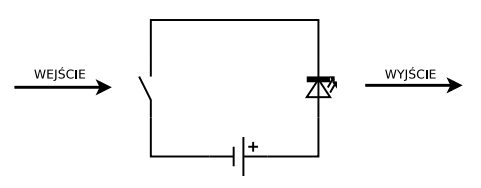
\includegraphics[scale=0.50]{./img/target_system/RT_wzorzec_led.png}}
Układ ten niewątpliwie spełnia wymagania systemów czasu rzeczywistego jednak w praktyce jest trywialny i zbyt ograniczony funkcjonalnie w przemysłowych zastosowaniach. Systemy którymi się zajmujemy posiadają układy mikroprocesorowe, dlatego stwórzmy odpowiednik tego trywialnego układu wykorzystując mikrokontroler.

 \centerline{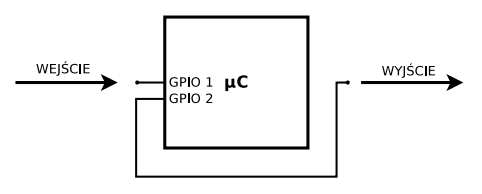
\includegraphics[scale=0.50]{./img/target_system/uc_RT_gpio.png}}
 
 Rozważany układ może pełnić rolę pokazanego wyżej prostego połączenia przełącznika do zewnętrznego odbiornika np diody led. Wejście mikrokontrolera jest wzbudzane sygnałem i system reaguje zmieniając stan wyjścia. W tym przypadku są to PIN-y GPIO ale sytuacja niczym się nie różni od wzbudzania wejścia przy pomocy innego (wewnętrznego mechanizmu). Np odczytywaniu stanu czujnika cyfrowego lub wartości napięcia, co w przypadku mechanicznego przełącznika byłoby niemożliwe. Systemy mikroprocesorowe dają nam dużo więcej możliwości niż układy oparte o mechaniczne rozwiązania, oraz co najważniejsze wypadają dużo lepiej w przypadku szybkich sygnałów niż jakiekolwiek mechaniczne zamienniki. Wymagają one jednak innego podejścia podczas testowania niż ich mechaniczne odpowiedniki ponieważ przebieg programu może być różny w zależności od warunków zewnętrznych. \\
 \centerline{\includegraphics[scale=0.10]{./img/target_system/rt_signal.png}}


\subsubsection{Definicja systemu RT na potrzeby pracy}

\par 
\tab Systemem czasu rzeczywistego w dalszej części pracy będziemy nazywali taki system operacyjny który spełnia wymagania określone jako "Hard real time" czyli dla każdej zdefiniowanej funkcjonalności posiada ograniczony z góry czasowy deadline.
Funkcjonalności są to w przypadku ogólnym wszystkie możliwe funkcje systemu których argumentami są zewnętrzne parametry. Funkcja taka musi dawać jakiś wynik, ponieważ musi być mierzalna. Funkcjonalności systemu mogą być wykorzystywane bezpośrednio przez użytkownika którym może być człowiek, inny system lub badane zjawisko.

\par
\tab Dodatkowo na potrzeby niniejszej pracy zakładamy, że każda z funkcjonalności jest przewidywalna czyli z góry znamy średni czas wykonania operacji. Przykładowo wiemy, że po naciśnięciu guzika w przeciągu pół sekundy zapali się dioda.
Kolenją cechą badanych dalej systemów czasu rzeczywistego jest wartość Jitter-a (wariacji opóźnienia) chcemy badać takie systemy w których Jitter nie jest funkcją losową a stanowi sumę różnych czynników zewnętrznych mających wpływ na wykonywanie operacji/funkcjonalności, z zastrzeżeniem że wartości tych czynników mogą mieć losową wartość w czasie (np wpływ promieniowania elektromagnetycznego w postaci fal radiowych na układ) jednak wartość ta jest ograniczona przez pewne normy (np normy dotyczące dopuszczalnego promieniowania elektromagnetycznego w mieście) lub ograniczenia przyrody (maksymalna/minimalna temperatura, wilgotność powietrza).

\par
\tab Powyższe założenia mają na celu wyodrębnienie takich systemów w których największe i znaczenie mają kwestię techniczne i inżynieryjne, natomiast nie skupia się na analizie opartej o zbyt głębokie matematyczne kwestię takie jak zaawansowana statystyka czy rachunek prawdopodobieństwa.

\clearpage
	\subsection{Charakterystyka systemu czasu rzeczywistego}

\newtheorem{master_thesis}{Postawiony problem}[section]

\subsubsection{Opis samodzielnego systemu RT}

\par 
\tab Budowa ogólna systemów mikroprocesorowych w tym systemów czasu rzeczywistego lub architektur sensorycznych jest do siebie bardzo zbliżona. Każdy system posiada blok sensorów które dają sygnały wejściowe, blok mikrokontrolera/procesora lub innej jednostki decyzyjnej (np: FPGA lub innych programowalnych układów) oraz blok wyjściowy do którego trafia wynik przetworzonych sygnałów z bloku sensorycznego. \\
Poniżej zaprezentowano ogólny schemat systemu wbudowanego który z jednej strony poprzez sensory wejściowe odbiera sygnały z otaczającego go środowiska, z drugiej strony poprzez blok wyjściowy jest w stanie reagować na przychodzące sygnały np: poprzez fizyczną zmianę sygnału elektrycznego, sterownik silnika lub wysłanie określonej wiadomości poprzez podłączone medium komunikacyjne takie jak układ radiowy czy internet. \\

 \centerline{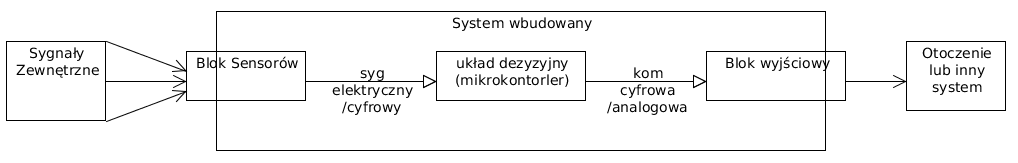
\includegraphics[scale=0.40]{./img/target_system/embedded_system_general.png}} 

\par
\tab
W przypadku systemów komunikujących się bezprzewodowo takich jak WSN blokiem wyjściowym oraz wejściowym jest układ radiowy służący do komunikacji z resztą systemu. Poniżej został przedstawiony schemat blokowy pojedyńczego węzła wchodzącego w skład bezprzewodowej sieci sensorycznej. \\

 \centerline{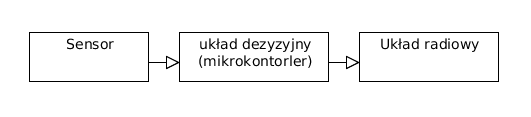
\includegraphics[scale=0.40]{./img/target_system/Uklad_badany.png}} 

\subsubsection{Przedstawienie badanego problemu}

\par 
\tab
Systemy czasu rzeczywistego w połączeniu z sieciami typu WSN wnoszą dodatkowy poziom skomplikowania ponieważ na szybkość odpowiedzi oprócz działania samego systemu operacyjnego wpływa również szybkość i niezawodność sieci w której odbywa się komunikacja między poszczególnymi węzłami. Jednakże takie połączenie wnosi bardzo wiele możliwości sprawiając że takie architektury mogą czerpać z największych zalet systemów RT oraz bezprzewodowych sieci sensorycznych. //
Przykładem takiego połączenia mogą być wszystkie interfejsy użytkownika wymagające odpowiedzi w czasie rzeczywistym takie jak np: bezprzewodowa kierownica, sterownik do urządzeń elektromedycznych, sterownik do zdalnie prowadzonych robotów i wiele innych zastosowań gdzie wyeliminowanie klasycznego połączenia kablowego wnosi wiele wygody, oszczędza miejsce czy daje możliwości lepszej pracy przy zachowaniu dotychczasowych cech czyli pewności działania, odpowiedzi w określonym czasie i bezpieczeństwa.

Celem niniejszej pracy jest zbadanie bezpieczeństwa systemu czasu rzeczywistego używającego do komunikacji sieci typu WSN na przykładzie bezprzewodowego włącznika do zastosowań medycznych. \\

\begin{master_thesis}
\textbf{ \textit{Analiza bezpieczeństwa bezprzewodowego włącznika nożnego do zastosowań  medycznych} }
\end{master_thesis}

Całość pracy obejmuje również elastyczną implementację takiego systemu w oparciu o różne systemy ogólno dostępne na rynku, która pozwoli na wnikliwą analizę wszystkich części składowych problemu.

Jako efekt pracy powstanie ocena przykładowej implementacji w ujęciu wymagań stawianych przez twarde systemy czasu rzeczywistego jakimi są niewątpliwie sterowniki urządzeń medycznych


\subsubsection{Opis domeny zagadnienia}

\par 
\tab Koncepcja wprowadzenia bezprzewodowych sterowników do urządzeń medycznych nie jest niczym nowym. Od czasu kiedy stały się popularne bezprzewodowe interfejsy użytkownika wszystkie branże zaczęły się zastanawiać czy w celu uzyskania dodatkowych profitów mogą wprowadzić bezprzewodowe interfejsy użytkownika, w zamian za istniejące kablowe/stykowe, do swojego biznesu. Dla zastosowań w których bezpieczeństwo i wysoka niezawodność transmisji nie jest krytyczną wytyczną rozwiązania te przyjęły się bardzo szybko, natomiast w branżach takich jak medycyna gdzie wytycznymi projektu rządzi bezpieczeństwo pacjenta i niezawodność urządzenia do tej pory najczęściej spotykanymi rozwiązaniami są połączenia za pomocą grubych kabli. \\

\tab Podczas mojej pierwszej pracy jako inżynier systemów wbudowanych w polskiej firmie prowadzącej sprzedaż urządzeń medycznych w tym laserów dużej mocy do zastosowań m.in. w chirurgii, pojawiła się koncepcja ułatwienia pracy chirurgom poprzez eliminacje rozmiarów urządzeń. Dla lekarzy problematyczne stały się ograniczenia wynikające z połączenia włącznika nożnego lasera za pomocą grubego kabla do głównego ciała urządzenia. Przewód elektryczny często był uszkadzany przez zgniatanie go innymi obiektami na sali zabiegowej, również połączenie przewodem utrudniało lekarzom komfort pracy ponieważ byli oni ograniczeni przewodem leżącym na podłodze przy stole zabiegowym który prowadził do lasera medycznego który często był niemobilnym urządzeniem przeznaczonym do umieszczenia w stałym miejscu. \\

\tab Ponieważ na pytanie czy wprowadzenie bezprzewodowego włącznika ułatwiłoby pracę i oczywiście skłoniło do zakupu, lekarze odpowiedzieli twierdząco firma postanowiła stworzyć takie rozwiązanie mimo tego że była to funkcjonalność rzadko spotykana na rynku dostępna tylko w niektórych urządzeniach. \\

Poniżej fotografia stosowanego przewodowego włącznika nożnego do zastosowań medycznych

 \centerline{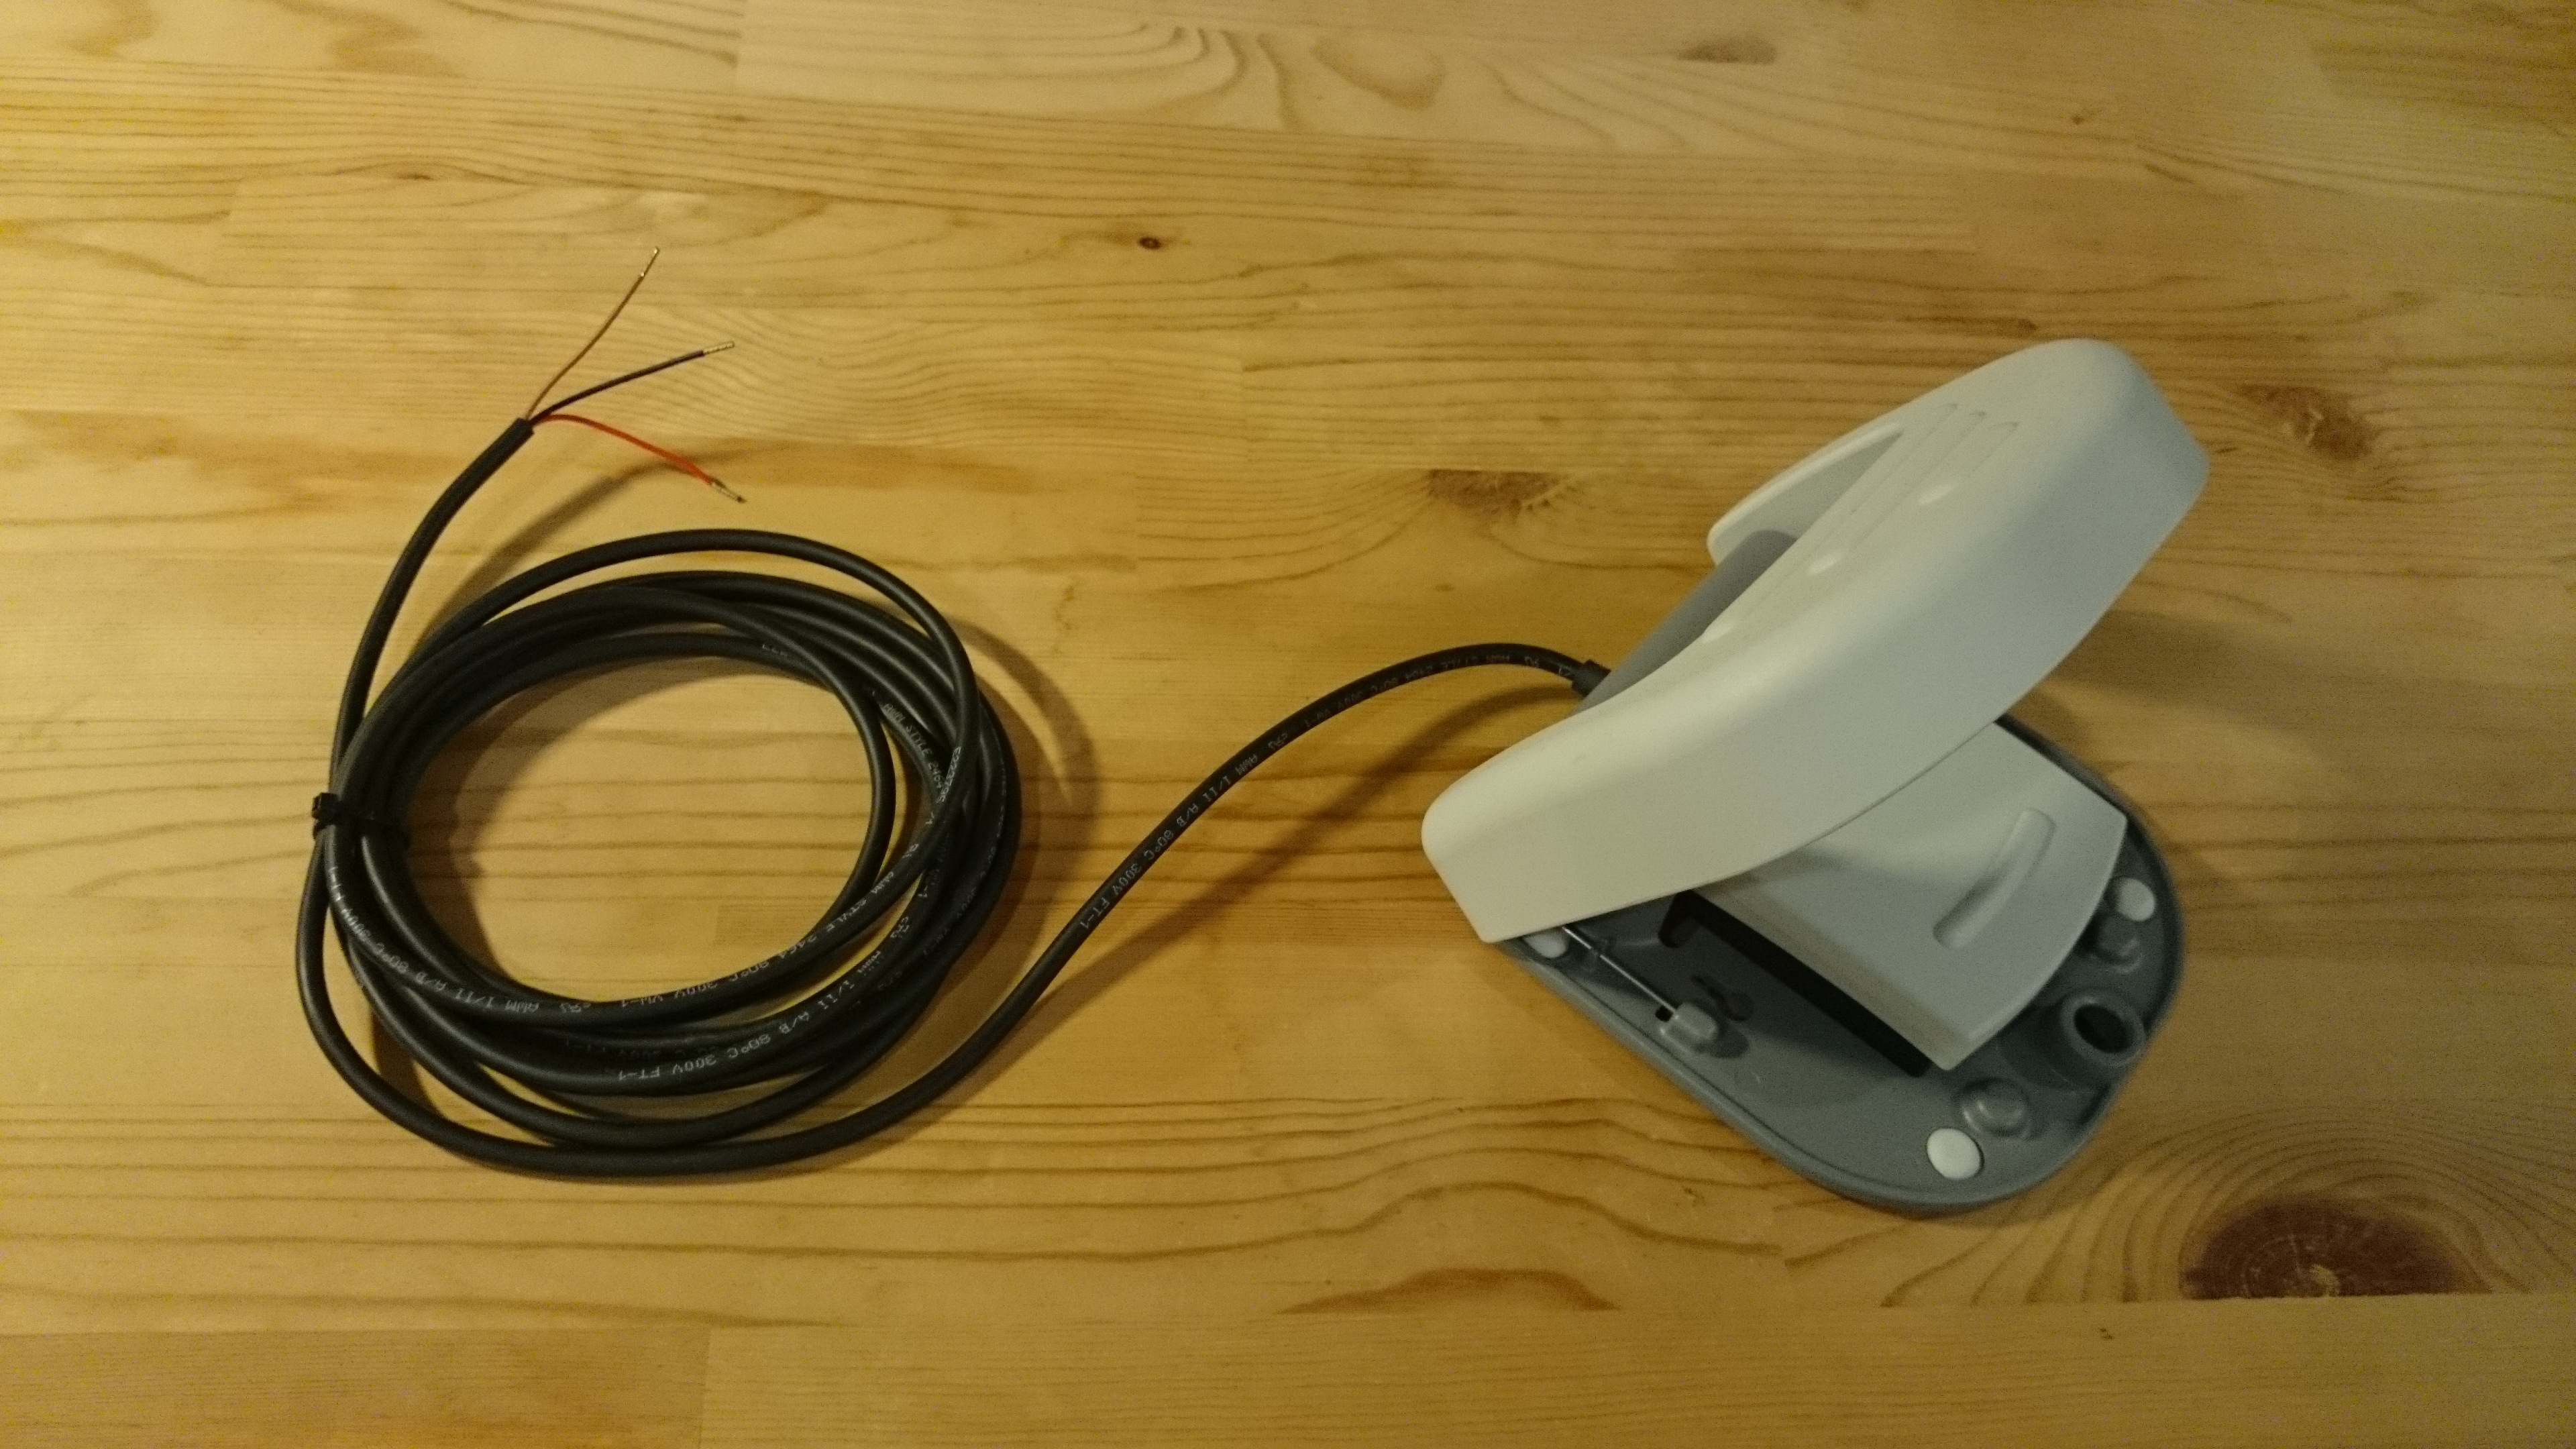
\includegraphics[scale=0.10]{./img/target_system/wlacznik_nozny.jpg}}

Oraz urządzenia lasera medycznego w tym przypadku jest to laser diodowy:

\centerline{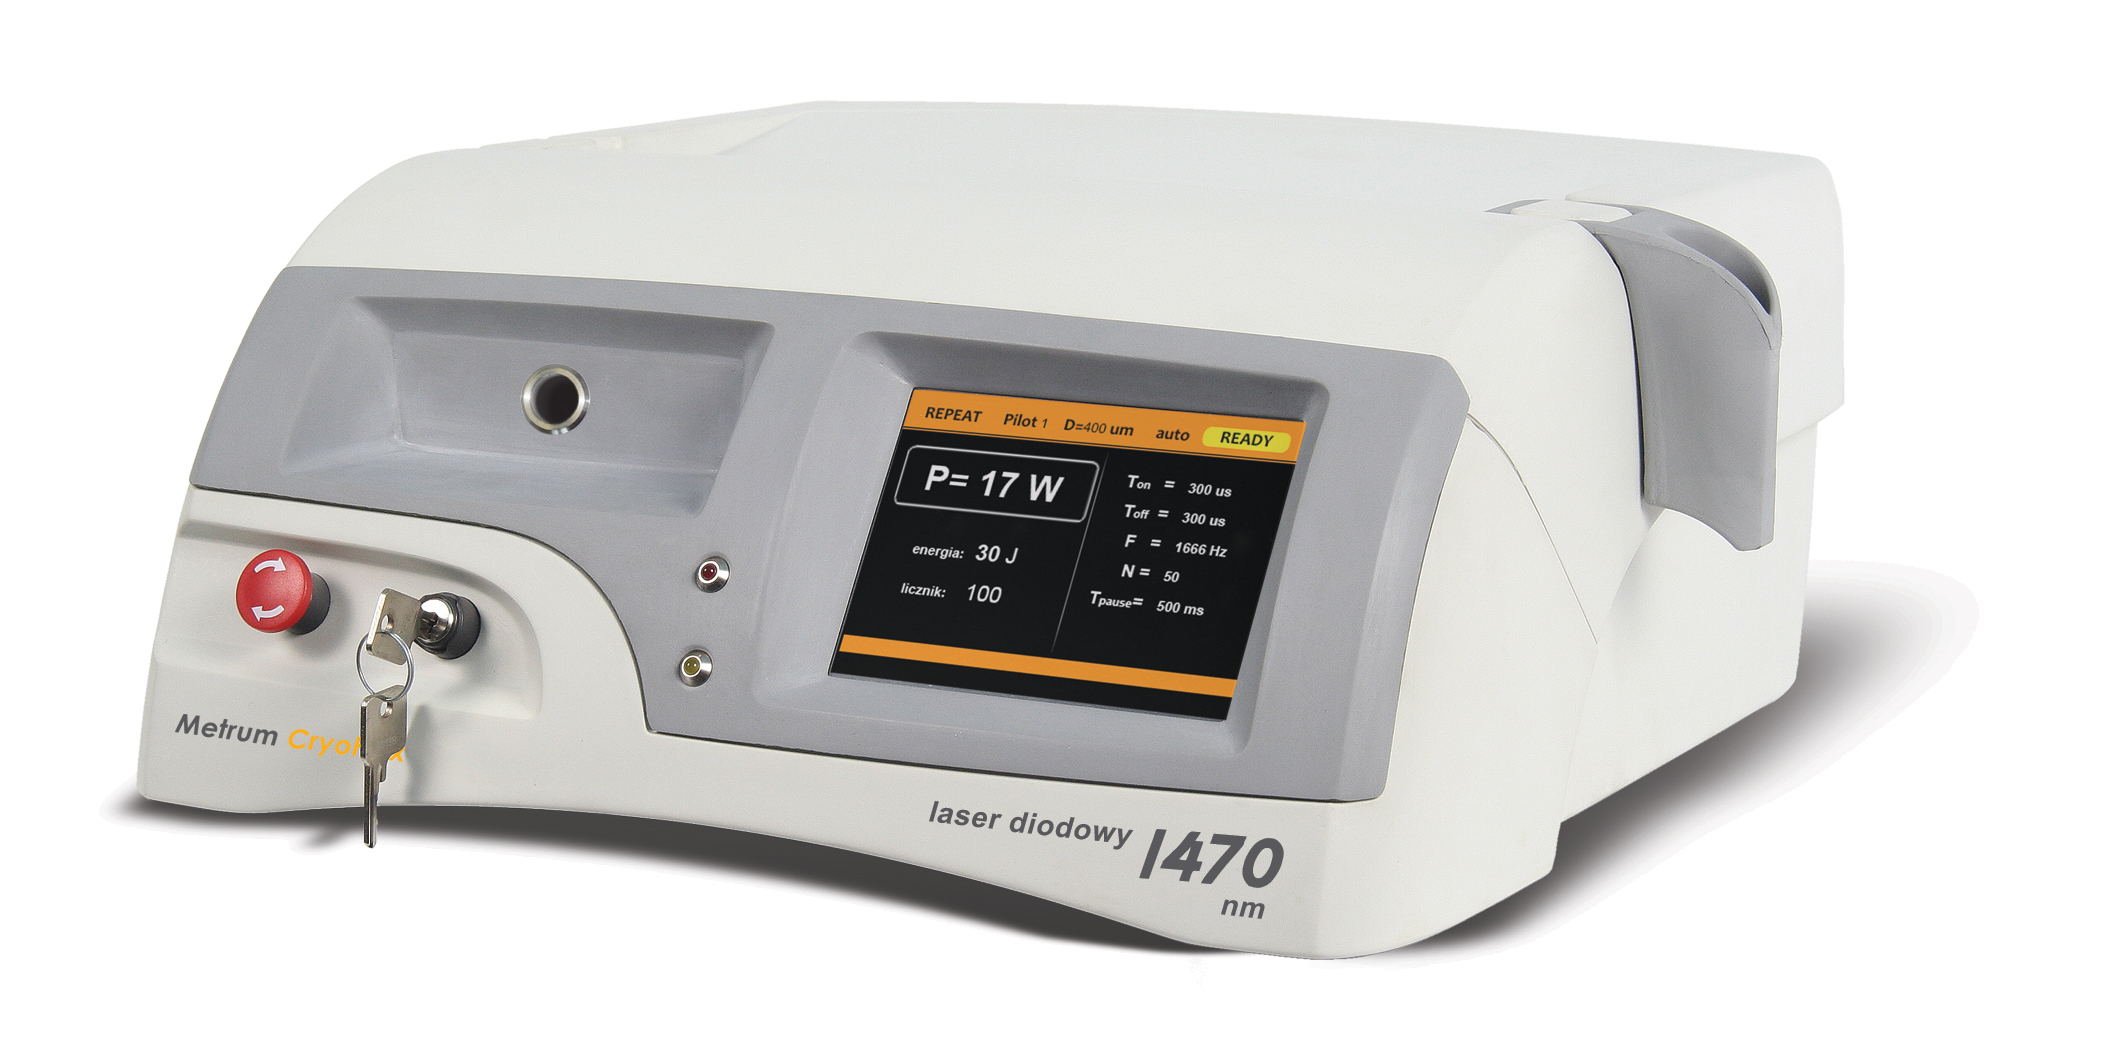
\includegraphics[scale=0.20]{./img/target_system/D1470_laser.jpg}} 

Jak widać laser jest dużym solidnym urządzeniem do którego od tyłu obudowy jest wczepiany włącznik za pomocą solidnego kabla o średnicy \diameter 6 mm. \\

\subsubsection{Analiza części składowych problemu} \mbox{}\\

Całość projektu systemu czasu rzeczywistego opartego o bezprzewodowe sieci sensoryczne można podzielić ogólnie na następujące częsci: \\

\begin{enumerate}
\item Ogólny projekt architektury systemu 
\item Wybór poszczególnych modułów systemu
\item Wyszczególnienie funkcjonalności czasu rzeczywistego
\item Stworzenie łańcucha procesu RT oraz zbadanie które moduły mają na niego wpływ
\item Przetestowanie łańcucha RT w zmiennych zewnętrznych warunkach 
\item Przetestowanie bezpieczeństwa systemu od zewnątrz i określenie potencjalnych niebezpieczeństw
\end{enumerate}

\paragraph{Ogólny projekt architektury systemu}\mbox{}\\
\tab W analizowanym przypadku system bezprzewodowego włącznika będzie składał się z dwóch węzłów: nadawczego który będzie zajmował się detekcją wł/wył oraz odbiorczego który będzie dawał sygnał do lasera medycznego o tym jaki jest obecnie stan włącznika.
Dla samego sterownika lasera jest niewidoczne skąd bierze się sygnał: czy z włącznika podłączanego kablem czy bezprzewodowego. Kontroler widzi jedynie zmieniający się stan wejściowy określający w jakim stanie jest włącznik.
\tab Oba węzły mają podobną budowę jak przykładowy węzeł z sekcji. -uklad badany

\centerline{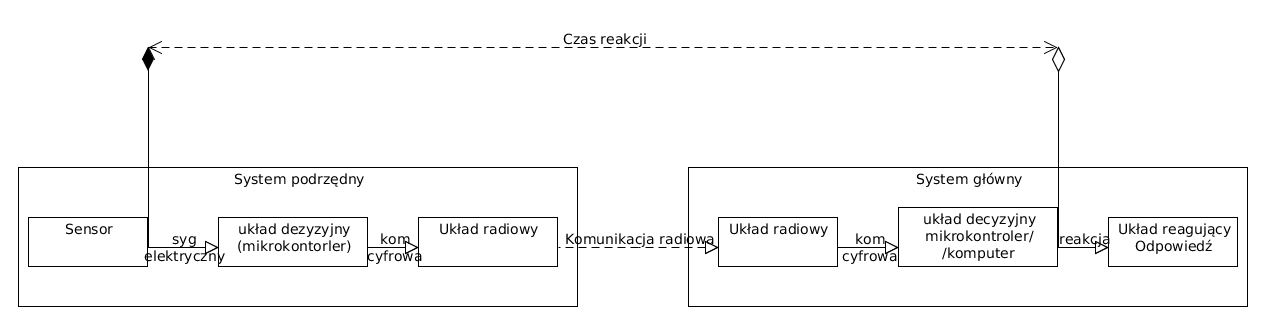
\includegraphics[scale=0.40]{./img/target_system/badany_system.png}} 

\paragraph{Wybór poszczególnych modułów systemu} \mbox{}\\
\tab W celu wyeliminowania z analizy elementów takich jak rózna implementacja standardów radiowych takich jak ZigBee lub BLE w projekcie zostanie użyty moduł typu OME czyli gotowy nadajnik z zaimplementowanymi warstwami protokołu radiowego.
Jako jednostka centralna zostanie użyty szybki mikrokontroler tak aby jego prędkość była pomijalna. Wybór padł na procesor ARM Cortex-M4 jako obecny standard przemysłowy dla systemów o średniej skali integracji.
System RT będzie również wybrany z pośród ogólnodostępnych standardów na rynku, ważną cechą przy tym wyborze jest otwartość kodu źródłowego oraz dobra dokumentacja.

\paragraph{Wyszczególnienie funkcjonalności czasu rzeczywistego} \mbox{}\\
\tab Każdy system elektroniczny posiada kilka standardowych funkcjonalności takich jak zarządzanie zasilaniem, przetwarzanie sygnałów przychodzących których źródłem mogą być dowolne czujniki dołączone do systemu.
Spośród wszystkich funkcjonalności często jako konstruktorzy systemu wyodrębniamy główne funkcjonalności, czyli najczęściej są to takie dla których de-facto tworzymy cały system. W Bezprzewodowych sieciach sensorycznych często spotykamy się z taką budową gdzie za jedną funkcjonalność odpowiada jeden węzeł sieci. \\
Przydładowo mając prostą sieć WSN do zastosowań w automatyce domowej dostarczamy klientowi następujące funkcjonalności: pomiar temperatur wewnątrz domu, na zewnątrz, sterowanie bramą wjazdową i włączaniem światła po zmroku gdy w pobliżu pojawi się mieszkaniec. Możemy śmiało spodziewać się 4 czujników które będą połączone radiowo i dodatkowo jakiejś jednostki głównej której funkcją jest zarządzanie siecią. O ile pomiar temperatury może nie wydawać się krytyczną kwestią o tyle sterowanie bramą wjazdową na posesję trzeba traktować jako funkcjonalność o najwyższym priorytecie ponieważ sytuacja w której zmęczony po całym dniu w pracy pan domu nie może otworzyć bramy wjazdowej pilotem i wjechać do domu bo właśnie następuje odczyt temperatury wydaje się być groteskowa. \\
Z tego powodu wszystkie funkcjonalności w systemie powinny być uporządkowane w pewnej hierarchii. 
W systemach czasu rzeczywistego główne funkcjonalności najczęściej są właśnie procesami czasu rzeczywistego, czyli takimi które muszą być obsłużone natychmiast po zaistnieniu nie zależnie od tego w jakim stanie obecnie znajduje się cały system.
Oprócz głównych funkcjonalności które czasem są nazywane mianem domenowych (czyli takich które decydują o branży w jakiej wykorzystywane jest całe urządzenie) występują jeszcze często nie zauważane przez użytkowników procesy o możliwym jeszcze wyższym priorytecie niż proces domenowy. \\
Przykładowo w naszym systemie czasu rzeczywistego bezprzewodowego włącznika nożnego stan włącznika (0-nie wciśnięty, 1-wciśnięty) musi być wiernie przeniesiony za pomocą drogi radiowej do ciała głównego lasera ponieważ ten sygnał będzie następnie odpowiadał stanowi włączenia wyłączenia Diody. Sam włącznik jest urządzeniem zasilanym bateryjnie z tego powodu warunkiem koniecznym do działania jest stan naładowania baterii, sytuacją nie dopuszczalną jest aby rozpocząć zabieg z baterią będącą na pograniczu wyczerpania ponieważ w tym momencie zachowanie całego włącznika mogłoby być nieprzewidywalne a więc również stan diody laserowej mógłby być nieprzewidywalny a sytuacja taka jest wysoce niedopuszczalna.
Kolejnym bardzo ważnym elementem całego systemu jest autoryzacja włącznika, czyli sprawdzenie czy włącznik komunikujący się z laserem jest dedykowany do tego lasera a więc tylko jeden włącznik może sterować jednym laserem i musi być to z góry określone.
Oprócz zastosowania mającego na celu zapobieganie \textit{Hakowania} systemu które nie mniej jest bardzo ważne, możemy sobie wyobrazić sytuację gdzie w dwóch gabinetach obok siebie pracują dwa lasery medyczne z bezprzewodowymi włącznikami. Aby system był bezpieczny te włączniki nie mogą na siebie oddziaływać. \\
 \centerline{W systemach RT Funkcjonalności możemy podzielić ze względu na: } \\
	\begin{itemize}
    	\item Krytyczność ze względu na czas
        \item Krytyczność ze względu na pełnioną funkcję
    \end{itemize}
    
Hierarchię między procesami określa się na początku tworzenia systemu na podstawie wymagań domenowych oraz technicznych. W naszym przypadku wszystkie funkcjonalności podzielimy na 3 grupy: Najwyższy priorytet, Wysoki priorytet oraz Niski priorytet. \\

   \centerline{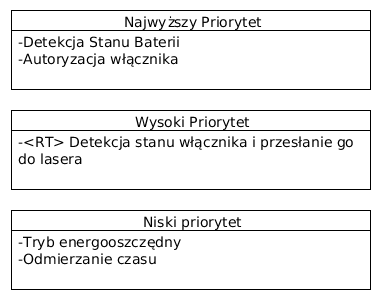
\includegraphics[scale=0.60]{./img/target_system/hierarchiaProcesow.png}} 


\paragraph{Stworzenie łańcucha procesu RT oraz zbadanie które moduły mają na niego wpływ} \mbox{}\\

\tab Głównym obiektem badań niniejszej pracy jest proces RT mający na celu przeniesienie stanu włącznika nożnego za pomocą fal radiowych na wejście lasera, która to włącza, wyłącza wiązkę lasera.
Jako argument wejściowy przyjmuje stan włącznika (wartość logiczna 0-1) a jako wynik zwraca również wartość logiczną. 
Matematycznie opisując przyjmujemy że x to stan włącznika a F(x) jest stanem przeniesionym bezpośrednio do ciała lasera: \\

\centerline{ $ F(x) = x  $ }

\centerline{  gdzie $  x, F(x) \in {-1,1} $ }

Na pierwszy rzut oka widać że funkcja jest trywialna i jedyne co robi to przenosi stan wejścia na wyjście jednak trzeba pamiętać że taki prosty model matematyczny nie uwzględnia opóźnienia które występuje w układzie i które badamy.
Następnie znając jakie są zależności wyjścia (F) od wejścia (x) należy rozbić na jednostkowe składowe przebieg całego procesu aby móc przeanalizować które elementy łańcucha wprowadzają opóźnienie i jakiego rodzaju jest to opóźnienie. \\
Poniżej znajduje się kompletny łańcuch z wyodrębnionymi elementami składowymi.\\

   \centerline{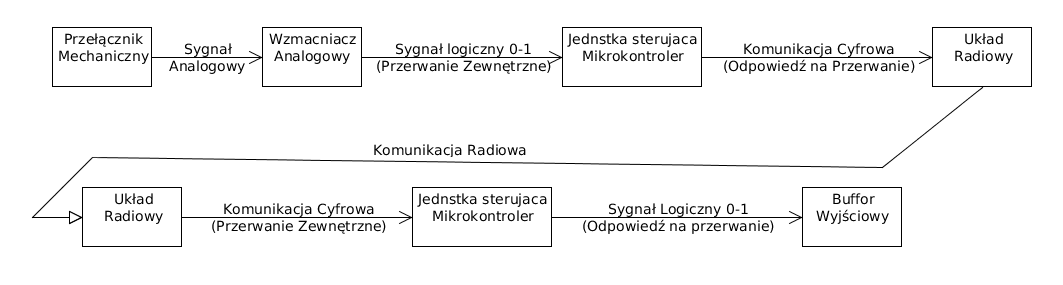
\includegraphics[scale=0.50]{./img/target_system/Lancuch_RT.png}} 

Idąc od lewej strony cały proces zaczyna się od przełącznika mechanicznego który w tym przypadku jest źródłem sygnału. Możemy sobie założyć że stan tego przełącznika określa dla nas czas zerowy czyli moment w którym cały proces się zaczyna z tego powodu taki przełącznik nie będzie wliczany do źródeł opóźnienia.\\
Następny element łańcucha czasu rzeczywistego to wzmacniacz analogowy. Ponieważ styki mechaniczne w momencie zwierania przez krótki ułamek czasu wprowadzają stan nieustalony pełen zakłóceń i drgań aby dokładnie wiedzieć w którym momencie nastąpiło fizyczne zetknięcie metali stosuje się filtry dolno przepustowe oraz wzmacniacz sygnału, ponieważ te dwie funkcjonalności można zrealizować za pomocą wzmacniacza operacyjnego przyjmujemy że jest to pojedyńczy blok. Ponieważ odpowiedź wzmacniacza operacyjnego w układzie filtru dolnoprzepustowego wyraża się w mikrosekundach możemy sobie przyjąć że ten blok ma pomijalnie mały stały czas który możemy zignorować (bardzo często w systemach czasu rzeczywistego pomijamy elementy elektroniczne analogowe ponieważ są one dużo szybsze od cyfrowych a ich czas jest stały) \\
Trzeci element łańcucha to mikrokontroler. W naszym przypadku uC działa pod wpływem tzw. RTOS (Real Time Operating System). Systemy takie mają tą zależność że ustawia się dla nich okres działania zegara systemowego (tzw. sys tick) który determinuje czas w jakim jest przewidywana zmiana wykonywania obecnego programu i obsługa funkcjonalności czasu rzeczywistego. Tutaj zostanie użyty standardowy czas dla tego typu systemów wynoszący 1ms, dzięki temu zyskujemy pewność, że maxymalnie w przeciągu 1ms od nastąpienia przerwania zewnętrznego zostanie uruchomiony kod który obsłuży to przerwanie. Z tego powodu dla mikrokontrolera należy przyjąć największe możliwe opóźnienie które wyniesie 1ms plus czas transmisji cyfrowej w celu nadania wiadomości radiowej do nadajnika.\\
Czwartym blokiem jest blok nadajnika radiowego, tutaj czas działania modułu jest zależny od wykonania przez producenta.
Blok ten łączy się z blokiem odbiorczym poprzez transmisję drogą radiową, dla ułatwienia w pierwszym podejściu możemy sobie przyjąć że będziemy traktować czas pomiędzy zleceniem transmisji wiadomości drogą radiową z jednego modułu RF do drugiego jako jeden czas, i jeśli będzie taka potrzeba to tenczas będziemy dalej rozbijać. \\
Przedostatni blok to mikrokontroler odbiorczy przyczepiony do ciała lasera tutaj mamy sytuację analogiczną jak w pierwszym uC.\\
Ostatni element łańcucha to bufor wyjściowy jest on analogiczny do wzmacniacza wejściowego, z tego powodu jego czas również możemy pominąć. \\
Podsumowując na całkowite opóżnienie składają się: \\

$ T_{calk} = T_{uC1} + T_{RFtransmit} + T_{uC2} $

$
 gdzie: \\
T_{uC1} \text{ : opóźnienie na wejściowym mikrokontrolerze} \\
T_{RFtransmit}  \text{ : opóźnienie podczas transmisji RF między nadajnikami} \\
T_{uC2} \text{ : opóźnienie na wyjściowym mikrokontrolerze } \\
$
\mbox{}\\

Dodatkowo czas transmisji radiowej możemy również rozbić na: \\

$ T_{RFtransmit} = T_{transmiterDelay} + T_{air} + T_{reciverDelay} $

$
gdzie: \\
T_{air} \text{ : rzeczywisty czas transmisji radiowej } \\
T_{transmiterDelay}  \text{ : opóźnienie na transmiterze } \\
T_{reciverDelay} \text{ : opóźnienie na odbiorniku } \\
$
\mbox{}\\

\paragraph{Przetestowanie łańcucha RT w zmiennych zewnętrznych warunkach } \mbox{}\\

W celu sprawdzenia czy zaprojektowany system posiada deterministyczną odpowiedź w czasie należy wykonać oczywiście odpowiednie testy polegające na mierzeniu czasu odpowiedzi na przychodzące zdarzenie w czasie. W naszym wypadku będziemy mierzyć czas od momentu pojawienia się sygnału odpowiadającemu wciśnięciu włącznika do momentu pojawienia się odpowiadającego mu sygału na wejściu lasera. \\
Ponieważ w obecnej postaci system jest modularny i umożliwia prostą zamianę jego modułów na inne zostaną przetestowane dwa standardowe protokoły radiowe wykorzystywane w sieciach typu WSN a mianowicie:
oparty o standard 802.15.4 protokół ZigBee oraz implementujący standard 802.15.1 Bluetooth Low Energy. \\
Czyli całe testy zostaną podzielone na dwie grupy:
\begin{itemize}
    	\item Testy sieci typu WSN opartej o ZigBee
        \item Testy sieci typu WSN opartej o Bluetooth Low Energy
    \end{itemize}
Dodatkowo testy będą się odbywać w otoczeniu innych nadajników nadających na tych samych częstotliowściach i kanale oraz dodatkowo w otoczeniu sieci Wifi która jest obecnie wszechobecnie występującą emisją elektromagnetyczną. \\
Testy opóźnień zostaną wykonane za pomocą oscyloskopa cyfrowego firmy ATTEN o prędkości próbkowania 50MHz i rozdzielczości 500MSa/s. Dla potrzeb testów przyjmiemy sobie jako podstawową jednostkę odniesienia pomiarów czasu 1ms z powodu standardu narzuconego przez system czasu rzeczywistego działający na mikrokontrolerze, oraz z uwagi na standardy transmisji cyfrowej których prędkość transmisji podawana jest w kB/s (1000 Bitów na sekundę) czyli w odniesieniu do mili sekundy. \\

\paragraph{Przetestowanie bezpieczeństwa systemu od zewnątrz i określenie potencjalnych niebezpieczeństw} \mbox{}\\

Oprócz głównej funkcjonalności jaką zapewnia system włącznika nożnego, system musi również spełniać inne wymogi wobec wymienionych wcześniej funkcjonalności o najwyższym priorytecie czyli: prawidłowej autoryzacji między urządzeniem lasera a włącznikiem, zarządzanie zasilaniem przez włącznik czy odporność na zakłócenia. \\
Testy systemu oprócz pomiaru samego czasu reakcji na zmieniony stan włącznika nożnego będą również obejmować: 
\begin{itemize}
    	\item Omówienie bezpieczeństwa sieci ZigBee/BLE oraz przedstawienie najnowszych badań dotyczących bezpieczeństwa sieci dla których będzie testowany system i odniesienie ich do zaprojektowanego systemu.
        \item Prównanie zużycia energi podczas transmisji samych modułów radiowych
        \item Wpływ zakłóceń na sieci WSN oparte o ZigBee/BLE, tutaj z wyszczególnieniem, że ten wpływ będzie jedynie omówiony ponieważ zbadanie samego wpływu eksperymentalnie wymaga specjalistycznego sprzętu oraz warunków laboratoryjnych.
    \end{itemize}

\subsubsection{Proponowane rozwiązanie}

\tab Nawiązując do schematu blokowego sieci WSN w punkcie poświęconemu ogólnemu projektowi architektury systemu omówimy poszczególne moduły systemu oraz ich implementację.\\

\paragraph{Wybór wzmacniacza}

Jako pierwszy omówimy blok wzmacniacza. Funkcją jaką ma on pełnić jest filtrowanie i wzmacnianie sygnału pochodzącego z mechanicznego przełącznika. Istnieje kilka rozwiązań spotykanych w przemyśle które odpowiedzialność za tę funkcjonalność przenoszą na mikrokontroler poprzez implementacje filtru cyfrowego lub poprostu przez tzw debouncing czyli w momencie wykrycia zmiany wprowadzenia sztucznego opóźnienia w celu ustalenia stanu wejścia i ponownym pomiarze. W systemach ukierunkowanych na czas oraz niezawodność staramy się przeprowadzać możliwie jak najwięcej obróbki sygnału w postaci analogowej, ponieważ czas jest nieporównywalnie krótszy a samo rozwiązanie dużo bardziej niezawodne. \\
Przy tworzeniu takiego filtra analogowego należy określić jego charakterystykę a najbardziej skupić się na paśmie które chcemy filtrować oraz wzmocnieniu. W naszym przypadku chcemy filtrować wszystkie szybkie sygnały głównie takie jak drganie styków oraz zakłócenia elektromagnetyczne. Interesuje nas wolnozmienny sygnał który powstaje w momencie zwarcia przełącznika mechanicznego.
W tym celu możemy sobie spokojnie przyjąć że chcemy ucinać wszystkie sygnały o wyższej częstotliwości niż 25Hz (punkt ten nazywany jest passband-frequency) dzięki takiemu pasmu wyeliminujemy również szkodliwy wpływ promieniowania sieci energetycznej 50Hz (lub 40Hz w innych częściach świata). \\ 
Drugim parametrem jest wzmocnienie dzięki któremu będziemy w stanie "uwidocznić" przychodzący sygnał.W naszym wypadku możemy to wzmocnienie ustalić wartość z przedziału 1-10 który jest standardowy w tego typu mechanicznych układach i ma na celu zniwelowanie niedoskonałości elementów oraz szkodliwy wpływ ewentualnych zanieczyszczeń. My wybierzemy wzmocnienie równe 5.
Mając już parametry filtra należy określić matematyczną charakterystykę, wybór ten polega na doborze istniejącego modelu na podstawie charakterystyki widmowej. Poniżej znajduje się kilka standardowych charakterystyk widmowych dla filtrów dolno-przepustowych o zadanych parametrach

\centerline{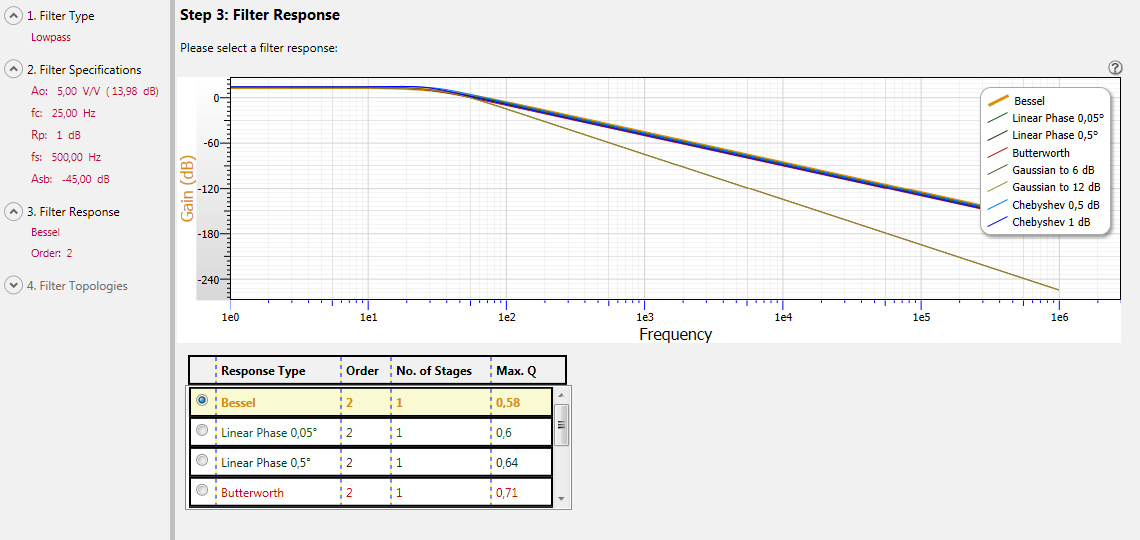
\includegraphics[scale=0.40]{./img/target_system/filtr/wybor_chrt_filtra.png}} 

Wyraźnie filtr bessla w tym porównaniu najlepiej wypada ponieważ jest on bardzo efektywny dla wolniejszych sygnałów. Tutaj także skorzystamy z niego. \\
Ważnym parametrem jest również stopień filtra, określa on zaz pomocą ilu fizycznych wzmacniaczy operacyjnych jesteśmy w stanie zbudować taki filtr, z tego powodu jeśli nie ma jakiś bardzo specjalistycznych wymagań należy wybrać charakterystykę o jak najmniejszej liczbie stopni. \\

Przykładowa budowa wzmacniacza operacyjnego dolno-przepustowego 2-giego stopnia w topologii Sallen-Key (standard w połączeniu elementów) wraz z charakterystykami fazowymi wzmocnienia oraz przesunięcia fazowego.

\centerline{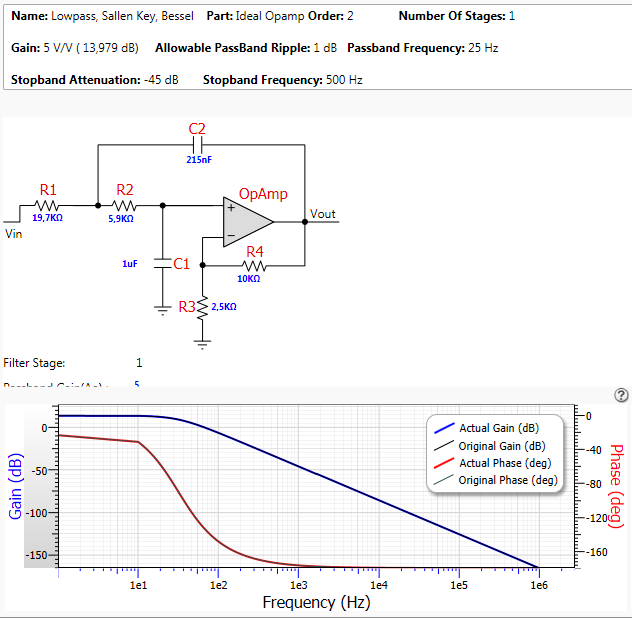
\includegraphics[scale=0.40]{./img/target_system/filtr/filter_design.png}} 

\paragraph{Wybór układu mikroprocesorowego i systemu RT}

Kolejnym elementem łańcucha czasu rzeczywistego jest układ mikrokontrolera. Obecnie panującym standardem na rynku mikrokontrolerów są układy zawierające rdzenie o architekturze ARM-Cortex. W naszym przypadku również skorzystamy z takiego układu ponieważ jest on ogólnodostępny w sprzedaży i istnieje wiele narzędzi wspierających pracę z takimi układami. Jako konkretny model wybór padł na układ firmy NXP LPC4330, należy on do rodziny mikrokontrolerów Cortex-M4 czyli najbardziej zaawansowanych układów z rodziny Medium Performance. Sam procesor LPC4330 ma możliwość działania na częstotliwości ponad 200MHz i jest on w momencie pisania tej pracy najszybszym ogólnodostępnym mikrokontrolerem w sprzedaży. \\
Wybór najszybszego mikrokontrolera pozwoli na zmniejszenie znaczenia prędkości wykonywania programu na mikrokontrolerze oraz kwestii technicznych związanych z budową samego układu peryferiów mikrokontrolera. Często konstruktorzy przypisują zbyt duże znaczenie do samej prędkości wykonywanego kodu podczas gdy największe opóźnienie rodzą się z powodu powolności transmisji, opóźnień związanych z odczytami z zewnętrznych układów. Do celów projektu zostanie użyta platforma ewaluacyjna dla mikrokontrolerów LPC4330 o nazwie \textit{"LPC4330-Xplorer"}
Na płytce ewaluacyjnej LPC4330-Xplorer oprócz micro-controllera znajduje się wiele ciekawych peryferiów takich jak przetworniki ADC do zastosowań audio, karta pamięci micro-sd, gniazdo i moduł ETH oraz porty we/wy w których skład wchodzi ponad 50 pinów GPIO pozwalających na podpięcie do modułu dowolnych peryferiów. Do portów tych zostanie podłączony wzmacniacz operacyjny oraz moduły radiowe służące do komunikacji między węzłami sieci. Płytka również posiada kryształ kwarcowy o dokładności +/-20ppm umożliwiający bardzo wysoką dokładność zegaru traktującego mikrokontroler.\\

\centerline{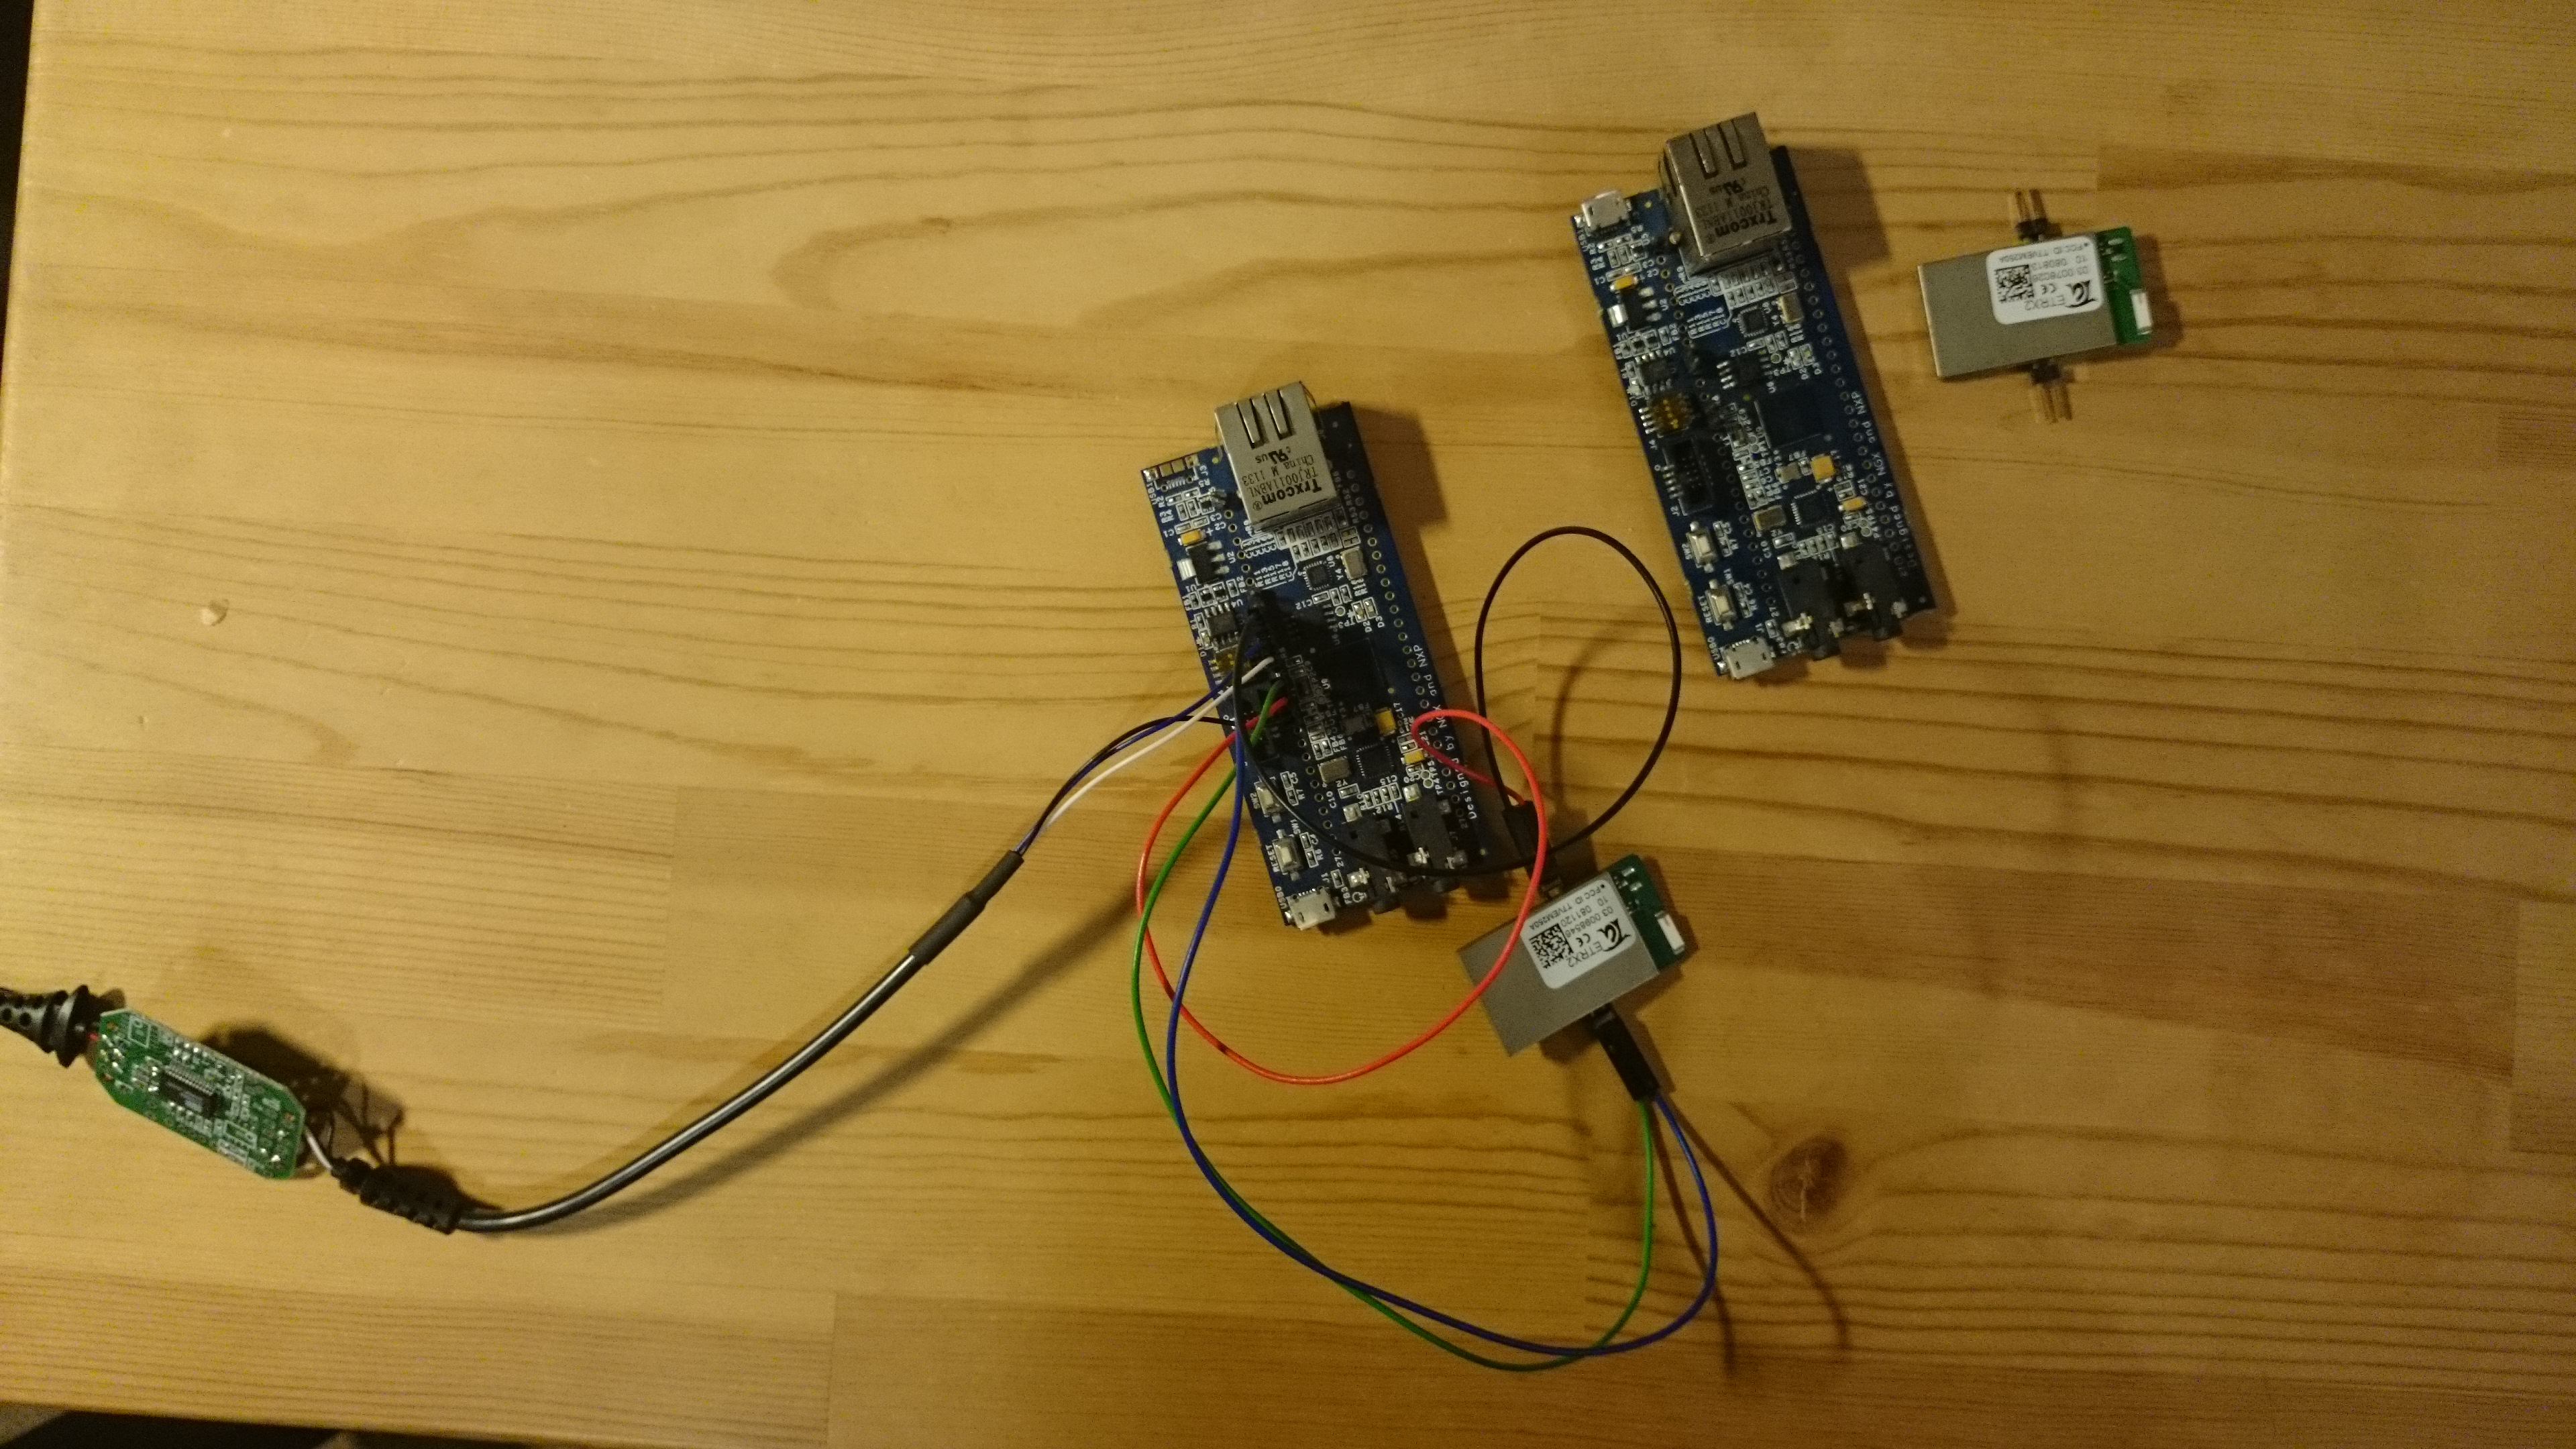
\includegraphics[scale=0.10]{./img/target_system/lpc4330-xplorer.jpg}} 

Do mikrokontrolera trzeba również dobrać odpowiedni system czasu rzeczywistego. W najprostrzym przypadku można stworzyć zwykły sekwencyjny program oparty o pętle główną (tzn. single-loop system), natomiast do bardziej skomplikowanych zastosowań często bezpieczniej jest użyć gotowego systemu. Na rynku istnieje wiele komercyjnych i otwartych RTOS-ów. W naszym przypadku posłużymy się otwartym systemem czasu rzeczywistego jakim jest projekt \textit{FreeRTOS}. \\
FreeRTOS jest systemem czasu rzeczywistego dostarczającym wszystkie najważniejsze funkcjonalności takie jak obsługa przerwań, planista, mechanizm kolejkowania czy priorytetyzacji zadań oraz również precyzyjne odliczanie czasu bez względu na obciążenie systemu.
Jest on również często używany jako standard rynkowy, ponieważ projekt jest otwarty i korzysta z niego wielu programistów na całym świecie. \\

\paragraph{Dobór układów transmisji radiowej}

Jak zostało wspomniane wcześniej, w ramach niniejszej pracy będziemy rozważać dwa typy transmisji radiowej opratej o standard ZigBee oraz BLE. Aby zrealizować taką transmisję należy skorzystać z odpowiednich układów radiowych oraz anteny. W naszym przypadku nie będziemy tworzyć od zera takiego modułu na podstawie gotowych układów, ale użyjemy już gotowych w pełni autonomicznych układów dostępnych na rynku. Podejście takie zwalnia nas z odpowiedzialności za samą implementację protokołu transmisyjnego oraz daje w zamian przyzwoitą prędkość transmisji ponieważ producenci takich układów często są specjalistami w dziedzinie technologii której dotyczą moduły możemy z powodzeniem przyjąć że prędkość komunikacji za pomocą modułu będzie wymierna ze zdefiniowanymi przez protokół standardami. \\
I tak jako układ komunikacyjny ZigBee zostaną użyte moduły ETRX3 firmy telegesis:

\centerline{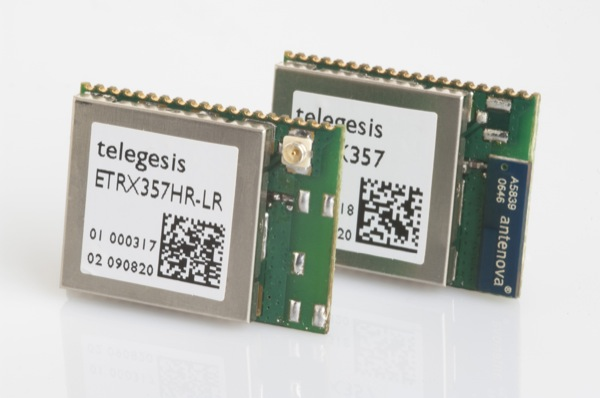
\includegraphics[scale=0.90]{./img/target_system/etrx3-modul.jpg}} 

Natomiast dla sieci Bluetooth smart moduł BLE112 firmy Bluegiga:

\centerline{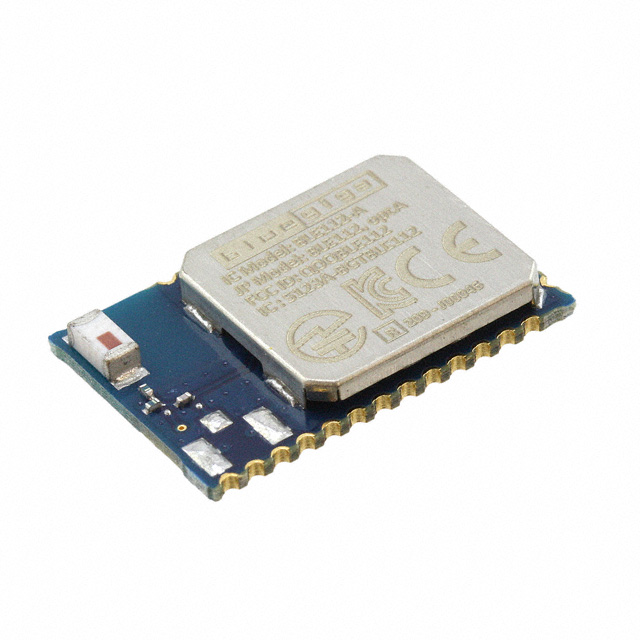
\includegraphics[scale=0.20]{./img/target_system/BLE112-module.jpg}} 

Obie firmy są liderami na rynku w zakresie komunikacji radiowej dlatego możemy sobie z pewnością założyć że wyniki osiągnięte przez ich moduły będą jak najbardziej adekwatne do implementowanych standardów.

\clearpage

	
	%Part 4
	\section{Przedstawienie wyników badań i ich omówienie}

\subsection{Polityka Bezpieczeństwa informacji}

W celu określenia czy dane rozwiązanie można nazwać bezpiecznym czy nie trzeba posłóżyć się pewną metryką. Sprawdzoną metryką jest tzw: \textit{Triada CIA - Confidentiality, integrity and availability}, pozwala ona na odniesienie dowolnego systemu informatycznego do modelu CIA poprzez analizę systemu/zasobów informatycznych w trzech wymiarach: poufności, integralności i dostępności.

\begin{enumerate}
	\item Poufność (\textit{Confidentiality}): Każdy system powinien mieć określone grupy odbiorców którzy mogą mieć dostęp do określonych danych. Poufność jest to cecha systemu informatycznego gwarantująca, że dane w systemie będą jedynie dostępne dla określonych osób/podmiotów i osoby trzecie (tzw. intruzi) nie będą w stanie poznaćtych danych. Ta włąściwość systemów informatycznych jest najczęściej zapewniana przez kryptografię.
	\item Integralność (\textit{Integrity}): Systemy komunikacyjne jak i również przechowujące dane muszą byś w stanie zapewnić integralność dostarczanych danych czyli innymi słowy być odporne na zgubienie danych czy dostarczenie uszkodzonych/niepełnych/przekłamnych danych. W systemach służących do komunikacji ta cecha jest najczęściej realizowana za pomocą podziału danych na pakiety i sprawdzaniu: czy pakiet jest nie uszkodzony oraz czy zależności między pakietami są właściwe (czy nie ma zgubionych lub nadmiarowych pakietów danych)
	\item Dostępność(\textit{Availability})): Główną funkcją wszelakich systemów informatycznych jest funkcja dostarczania danych do odbiorcy. Dostępność gwarantuje nam, że po wysłaniu prawidłowego żądania dostępu do danych otrzymamy je w skończonym-określonym czasie.
\end{enumerate}

\par
\tab Ponieważ opisany wcześniej System RT jest systemem krytycznym ze względu na funkcję \textit{(przyp. Sterowanie Laserem Medycznym przeznaczonym do wykonywania zabiegów na ludziach)} \\
Aby zbadać czy zbudowany System RT jest \textit{"Bezpieczny"} zmierzymy go w wymiarach: Poufności, Integralności oraz Dostępności danych. Następnie na podstawie tych wyników spróbujemy określić czy spełnia on wymogi bezpieczeństwa modelu CIA. \\
Aby określić co tak naprawdę musi zostać zbadane należy przyporządkować do właściwości C-I-A określone moduły, właściwości danych:
\begin{enumerate}
	\item Poufność - Wiąże się bezpośrednio z szyfrowaniem danych wysyłanych w pakietach oraz z kwestiami takimi jak ustalenie bezpiecznej sesji czy działaniem mechanizmów komunikacyjnych protokołu. W celu ustalenia czy system spełnia dane wymogi poufności w dalszej części zostanie przeprowadzona analiza bezpieczeństwa dla rozwiązania opartego o protokół komunikacyjny ZigBee oraz BLE.
	\item Integralność - Za tę właściwość odpowiadają warstwy fizyczne protokołu (W wypadku Zigbee - protokół 802.15.4 natomiast dla BLE 802.15.1) ponieważ ta właściwość jest określona przez sam protokół i zapewniona za pomocą stosownych mechanizmów takich jak np. CRC dla każdego pakietu czy stos protokołu, nie będzie ona w ramach niniejszej pracy szczegółowo badana.
	\item Dostępność - Zależy bezpośrednio od tego jak szybko jest w stanie odbiornik odpowiedzieć na żądanie przychodzące z nadajnika. Jest to również jedna z cech systemów real-time. Aby sprawdzić czy system spełnia wymogi dostępności w kolejnej części zostaną przedstawione wyniki eksperymentu oraz ich analiza.
\end{enumerate}

W dalszej części zostaną przedstawione wyniki "Analizy czasowej systemu RT" oraz "Analiza podatności i zagrożeń dla protokołów ZigBee i BLE". Następnie w odniesieniu do modelu CIA zostanie określone czy dany System-RT jest \textit{Bezpieczny} czy nie, a ponieważ niniejszy system RT jest systemem wzorcowym i modularnym, na jego podstawie będzie można zadecydować czy inny system opierający się o protokół komunikacji BLE/ZigBee może być bezpiecznym, ponieważ analiza będzie ogólna.

\clearpage
	\subsection{Analiza czasowa procesu RT}

\par
\tab W celu zweryfikowania czy dany proces systemu spełnia wymagania \textit{Twardych systemów czasu rzeczywistego} stworzony został układ pomiarowy mający na celu badanie odstępu czasowego między pojawieniem się sygnału na wejściu a zmianą stanu wyjścia układu. \\ 


\begin{wrapfigure}{r}{0.5\textwidth}
  \vspace{-20pt}
  \begin{center}
    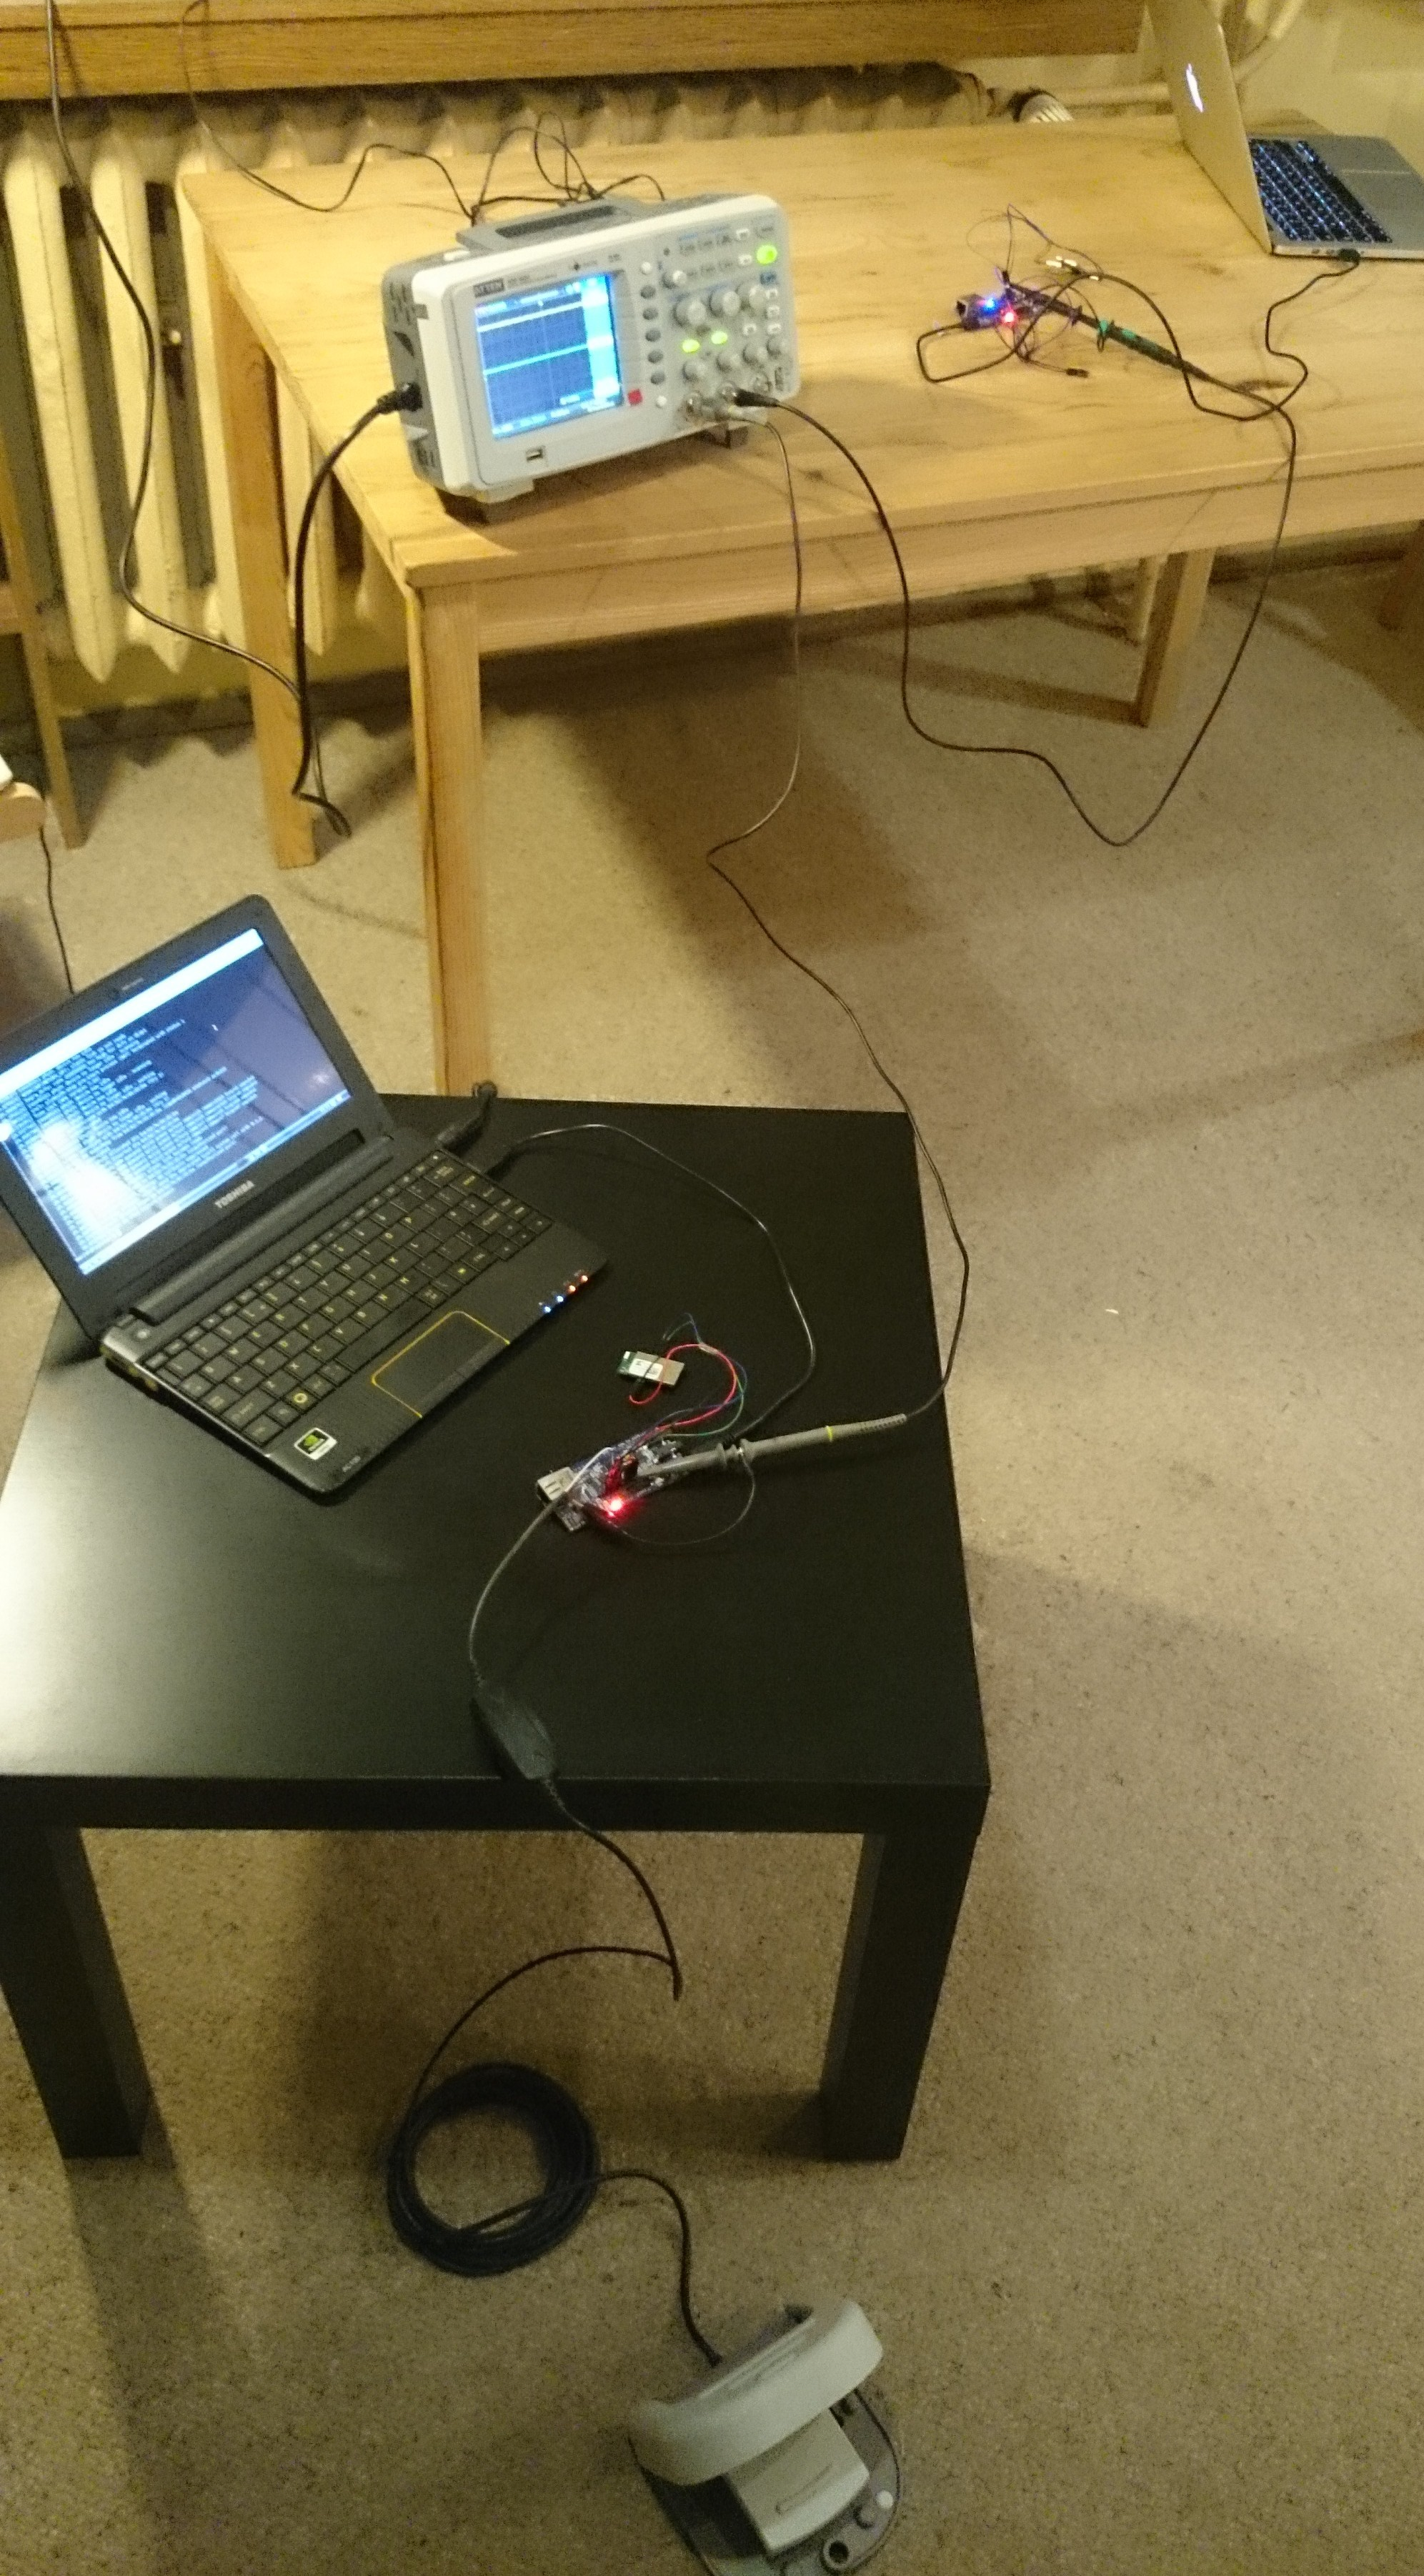
\includegraphics[scale=0.10]{./img/target_system/response_measure.jpg}
  \end{center}
  \vspace{-10pt}
\end{wrapfigure}

W tym celu dwa układzo stały rozmieszczone w odstępie od siebie odpowiadającym przykładowej docelowej odległości, następnie układ detekcji włącznika był regularnie pobudzany na wejściu sygnałem imitującym zwarty włącznik. \\
\tab Dzięki zastosowaniu nadajników RF w postaci gotowych modułów w prosty sposób można w takim układzie przetestować oba rozwiązania oparte o Zigbee i BLE. \\

\par
\tab Wykonano 3 rodzaje testów: 2 typy dla Zigbee poniważ dysponuje ona zmienną długością pakietu danych od 1 bajtu do 72. Z tego powodu wykonano 2 serie pomiarów dla transmisji 1 bajta oraz 72 bajtów. Bluetooth Low energy umożliwia natomiast transmisję do 20 bajtów, z tego powodu została przetestowana transmisja dla długości danych w pakiecie wynosząca maksymalną długość. \\
Również należy wspomnieć że badany czas jest sumą czasu samej transmisji radiowej oraz czasu odpowiedzi systemu RT znajdującego się w mikrokontrolerze, ma on ustawiony sprzętowy zegar o częstotliwości 1kHz (okres 1ms), steruje on planistą systemowym co oznacza ze czas na uruchomienie odpowiedniego zaadania w mikrokontrolerze od czasu jego wyboru wyniesie zawsze nie więcej niż 1ms. (Należy pamiętać, że zegar systemowy nie ma niczego wspólnego z prędkością traktowania jednostki centralnej która jest dużo wyższa i decyduje o częstotliwości rdzenia). Dodatkowo każdy z radiowych modółów ma w sobie również microprocesor do prowadzenia transmisji który również wprowadza pewne nieznaczne opóżnienie.\\ 
Ze względu na rozdzielczość zegara systemowego wynoszącą 1ms do pomiarów zostały zastosowane 3 odcinki czasu: 0-1ms, 1-5ms oraz 5-10 ms. Górna granica 10ms wynika z faktu że podczas sesji pomiarowej (wynoszącej 1000 pomiarów) najdłuższe czasy oczekiwania wypadły do ok 9 ms.
Poniżej przedstawiono zestawienie danych pomiarowych w tabeli:
\mbox{}\\
\begin{tabular}{ |p{3cm}||p{3cm}|p{3cm}|p{3cm}|  }
 \hline
 \multicolumn{4}{|c|}{Ilość Zmierzonych transmisji na 1000 prób} \\
 \hline
 Rodzaj transmisji & Tresp 0-1 ms & Tresp 1-5 ms & Tresp 5-10 ms\\
 \hline
 Zigbee, wielkość ramki 1byte   & 231    & 748 &   21\\
 Zigbee, wielkość ramki 72bytes &   0  & 863   &137\\
 BLE, wielkość ramki 20bytes &0 & 882&  118\\
 \hline
\end{tabular}
\mbox{}\\
\par
\tab Należy zwrócić uwagę, że mierzony czas stanowi sumę czasów obsługi przerwania przez mikrokontroler oraz transmisji radiowej przez modół RF.
Teoretyczną długości czasu transmisji radiowej można zgrubnie oszacować poprzez skorzystanie z danych pochodzących ze standardu: \\

\begin{enumerate}
\item Dla Bluetooth Low Energy taka prędkość transmisji wynosi do 3ms i jest określona przez standard Bluetooth 4.0
\item Dla transferu 1 bajta za pomocą protokołu ZigBee czas transmisji jednego bitu wynosi wg standardu 32 us. Przy transferze 1 bajtu pakiet zawiera również 25 bitów czyli w sumie całkowity czas wynosi: (25 + 1) * 32 us = 0.83 ms.
\item Dla transferu 72 bajtów czyli największej dopuszczalnej przez standard ZigBee w wersji 2 wyniesie (13 + 72) * 32 us = 2.72 ms
\end{enumerate} 

\par
\tab Jak widać na powyższych wynikach przy założeniu czasowego deadlinu wyszącego 20ms system spokojnie może pełnić funkcję RT. 20ms z punktu widzenia człowieka to ułamek sekundy a dla systemu 2-krotnie większa wartość daje margines bezpieczeństwa.

\clearpage
	
\subsection{ Analiza kwestii bezpieczeństwa i przedstawienie znanych zagrożeń. }

\par
\tab W tej części zostaną przeanalizowane na dzień dzisiejszy znane podatności zarówno sieci opartych o protokół ZigBee jak i o Bluetooth Low Energy. Ponieważ obydwa rozwiązania jako swój fundament zakładają niski pobór energii przez podłączony węzeł, naturalną kwestią jest to, że obliczeniowo węzły nie są na dzień dzisiejszy implementować rozwiązań znanych z kryptografii asymetrycznej oraz bezpiecznych protokołów takich jak TLS czy SSL.\\
W zamian natomiast twórcy obu protokołów dołożyli największych starań aby oba te protokoły były jak najbardziej bezpieczne. \\

\par
\tab \textbf{ Bluetooth smart: \textit{"With low energy comes low security"}  }\\

Przeszukując sieć w poszukiwaniu narzędzi do ataku na Bluetooth Low Energy zetkniemy się napewno z najbardziej znanymi a mianowicie: projekt \textit{Ubertooth} oraz dobrze znany analizator pakietów sieciowych \textit{Wireshark} posiadający opcję analizy zarówno pakietów Bluetooth jak i również BLE.

	Na podstawie obecnych badań znanych jest kilka podatności sieci BLE, najbardziej znane to:
\begin{enumerate}
	\item Sniffing komunikacji
	\item Obchodzenie procesu parowania urządzenia
	\item Reużywanie tego samego klucza sesji	
\end{enumerate} 

\par
\tab \textbf{ "Sniffing Bluetooth Le is not hard" czyli o Sniffingu. }\\
-Powyższe hasło pochodzi z jednej z konferencji poświęconych bezpieczeństwu elektronicznemu, nawiązuje ono do hasła ktore stało się motywacją dla projektu Ubertooth[*]: "Sniffing Bluetooth is hard".\\
Jak zostało wcześniej wspomniane BLE jako protokół prowadzi transmisję na jednym z 37 kanałów transmisyjnych do wymiany danych, oraz korzysta z Techniki Hopping-u (po każdej wymianie pakietu zmienia kanał na numer obliczony poprzez dodanie wartości \textit{Hop Increment} do obecnego numeru) \\

\centerline{ $ NextChannel \equiv curren channel + hop increment (mod 37) $ } 
\mbox{}\\
Przykład komunikacji przy \textit{Hop Increment = 7} 
\mbox{}\\
\mbox{}\\
\centerline{ $ 3 \to 10 \to 17 \to 24 \to 31 \to 1 \to 8 \to 15 \to ... $ } 
\mbox{}\\
Algorytm Snifowania: 
	\begin{enumerate}
\item Ustaw częstotliwość odczytu na następny kanał
\item Następnie podąrzaj za transmisją uwzględniając hop inc
\end{enumerate} 
\mbox{}\\
\tab W celu przeprowadzenia takiego snifinu są wymagane jeszcze zmienne bezpośrednio związane z protokołem komunikacyjnym na którym posłuchujący chce odczytywać dane z kanału, a których to na początku nie zna: \textit{AccessAddress, CRCInit, Hop Interval, Hop Increment}. \\
Aby uzyskać AccessAddress należy skorzystać z faktu że w protokole wymieniane są puste pakiety które nie zawierają danych a służą jedynie do synchronizacji wymaganej przez hop internal. Taki pusty pakiet oprócz pustej liczby bitów posiada szukany adres. \\
CRCInit jest inicjalizującą sumą kontrolną na podstawie której obliczane jest CRC która służy do sprawdzania poprawność pakietu. Ponieważ liczenie CRC działa na podstawie rejestru przesuwającego z liniowym sprzężeniem zwrotnym da się je odzyskać odwracając tę liniową operację ["Bluesniff: Eve meets Alice and Bluetooth”, USENIX WOOT '07] \\
\tab HopInterval pozyskać można poprostu wyczekując na tym samym kanale 2 kolejnych pakietów z tym samym adresem. Ponieważ liczba 37 jest liczbą pierwszą mamy pewność, że niezależnie od kanału po pewnym czasie transmisja nastąpi na tym kanale.

\centerline{ $ \frac{\Delta t}{37 x 1.25 ms} = hop interval $ }
\mbox{}\\
Hop Increment można bardzo łatwo uzyskać po tym jak się otrzymało HopInterval, wystarczy poczekać na kanale 0 na transmisję a następnie wyczekiwać momentu w którym pojawi się pakiet na kanale 1-szym.
Ponieważ znamy HopInterval więc możemy policzyć jak dużo kanałów zostało przeskoczonych pomiędzy 0 i 1.
\mbox{}\\

\begin{gather*}
        0 + hopIncrement × channelsHopped  \equiv 1 (mod 37)\\
        hopIncrement \equiv  channelsHopped^{-1} (mod 37) \\
        channelsHoppped^{-1} \equiv channelsHopped^{37-2} (mod 37)
\end{gather*}

W efekcie czego otrzymujemy wszsytkie parametry połączenia które możemy zawsze w przyszłości śledzić ponieważ BLE domyślnie zapamiętuje parametry transmisji z urządzeniem aby w kolejnych komunikacjach nie marnować energii na ustalanie ich od początku. \\

\par
\tab \textbf{Obchodzenie mechanizmu parowania} \\
Jak wcześniej zostało wspomniane Bluetooth Low Energy w standardzie obsługuje mechanizm symetrycznego szyfrowania w oparciu o Algorytm szyfrujący AES - 128bitowy. Szyfrowanie odbywa się na warstwię łączącej (Link Layer) protokołu. Podczas procesu następuje szyfrowanie części pakietu PDU (Dla zobrazowania tego faktu poniżej została zaznaczona omawiana część pakietu na czerwono), natomiast pozostała część jest przesyłana w postaci jawnej.\\

\centerline{
	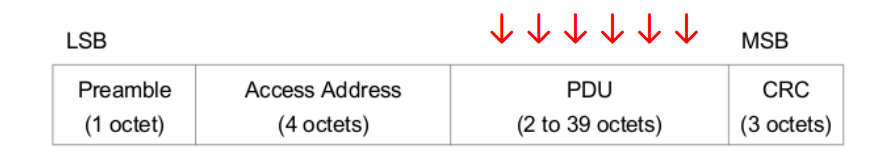
\includegraphics[scale=0.35]{./img/AES_PDU_crypt.png}
}
Trzy metody parowania urządzeń BLE
\begin{enumerate}
	\item Parowanie bez PIN-u
	\item 6 cyfrowy PIN
	\item PIN 00B	
\end{enumerate} 

\tab W celu przeprowadzenia szyfrowanej transmisji musi najpierw zostać wykonany proces wymiany klucza, nazywany potocznie parowaniem. Proces ten jest trójstopniowy, i podczas niego na początku obie strony uzgadniają między sobą TK (temporary key) poprzez 3 etapową wymianę danych za pomocą 3 parametrów: rand (liczba pseudolosowa), p1/p2 (parametry zależne od pinu, dla 00B są to zera). Parametry te są przesyłane między stronami \textbf{postaci jawnej w powietrzu}, za pomocą tych wartości obie strony wyliczają tzw \textit{confirm value}, po wyliczeniu którego komunikacja między stronami zaczyna być szyfrowana za pomocą TK, a następnie jest w ramach sesji STK (Short term Key) który służy do ustawienia bezpiecznego połączenia w ramach którego może być przesłany LTK (Long Term Key) którego w przyszłości strony będą używać do komunikacji.
Jednakże posiadająć TK, można odszyfrować STK oraz sesję a w efekcie czego LTK

Sposób rozszyfrowywania TK
\begin{gather*}
        configm = AES(TK, AES(TK, rand XOR p1) XOR p2)\\
        confirm, rand, p1/p2 są przesyłąne w postaci jawnej \\
        TK jest wartością od 0 do 999,999 dla PIN6 lub 0 dla JustWorks
\end{gather*}


\par
\tab \textbf{Reużywanie tego samego klucza sesji} \\

\tab Po tym opisie łatwo wywnioskować, że żadna z powyższych metod parowania nie zapewnia ochrony przeciwko pasywnemu podsłuchiwaniu. \\
Mało tego ponieważ protokół bluetooth LE był projektowany dla urządzeń wbudowanych zasilanych bateryjnie protokół uwzględnia mechanizm \textit{Counter-mitigation} który ma na celu zapewnienia możliwości ponownego uzgodnienia klucza w przypadku gdyby któreś z urządzeń straciło pamięć w wyniku rozładowania baterii. Skutkuje to możliwością podsłuchującego do wymuszenia celowej renegocjacji klucza, nawet gdy oba urządzenia zostały już poprawnie sparowane w bezpiecznym miejscu.
Atakujący który raz podsłucha procesu parowania jest w stanie odtworzyć TK, STK oraz LTK. 
Samo ustalenie TK za pomocą metod typu bruteforce zajmuje mniej niż 1 sekunde na 1 rdzeniu procesora intel i7 który nie ma sprzętowego wsparcia dla algorytmu AES, i umożliwiają to powszechnie dostępne w sieci narzędzia OpenSource. \\


\par
\tab \textbf{ ZigBee: \textit{and KillerBee}  }\\

Podobnie jak w przypadku poprzedniej części zostaną wymienione znane techniki ataków na sieci ZigBee, łącznie z omówieniem zasad ich działania.
Materiałów dotyczących samych podatności sieci ZigBee jest dużo mniej niż w przypadku innych protokołów bezprzewodowych ponieważ sam standard nie jest na tyle popularny w życiu codziennym jak ma to miejsce przy np 802.11 (Wifi) czy Bluetooth i BLE. Z otwartych narzędzi służących exploitacji oraz sniffingu protokołu ZigBee warto wymienić framework KillerBee czy narzędzie WireShark posiadające opcję sniffingu i analizy pakietów ZigBee.
Specyfikacja ZigBee zawiera w sobie szereg elementów przewidzianych do tego aby chronić \textit{"Poufności oraz integralności danych"}, głównymi z nich jest używanie standardu kryptograficznego AES oraz Autentykacji danych za pomocą klucza sieciowego. Dodatkowo standard ten definiuje dwa tryby bezpieczeństwa:
\begin{enumerate}
	\item \textbf{Standardowy tryb bezpieczeństwa} \textit{(Standard security mode)}: w którym to autentykacja każdego węzła odbywa się za pomocą współdzielonego klucza sieciowego dostarczanego i uwierzytelnianego przez Trust Center oraz Listy dostępu \textit{ACL (Access Control List)}
	\item \textbf{Tryb wysokiego bezpieczeństwa} \textit{High security mode} w tym trybie autentykacja jest dużo bardziej restrykcyjna ponieważ Trust Center trzyma wszystkie klucze szyfrujące oraz autentykujące używane w sieci. Z tego powodu musi dysponować one dodatkowymi zasobami aby być w stanie śledzić wszystkie urządzenia w sieci oraz odmawiać niechcianym urządzenią dostępu do sieci.	
\end{enumerate} 

Na podstawie obecnych badań oraz materiałów znane są następujące ataki na sieć ZigBee:
\begin{enumerate}
	\item Odkrywanie fizycznego połorzenia węzłów
	\item Sniffing pakietów
	\item Wstrzykiwanie pakietów
	\item Przechwytywanie transportu klucza (Tylko sieci w trybie Standardego trybu bezpieczeństwa)
\end{enumerate} 


\par
\tab \textbf{Odkrywanie fizycznego połorzenia węzłów} \\
Wszystkie układy radiowe które są emiterami emitują pole elektromagnetyczne. W przypadku standardu 802.15.4 układ radiowy może jako część protokołu zeskanować sieć i dla każdego odnalezionego adresu w sieci wyznaczyć jego siłę sygnału. Takie rozwiązanie jest bardzo pomocne przy tworzeniu sieci, debugowaniu czy diagnostyce, jednakże umożliwia ono również każdemu wyposażonemu w układ radiowy intruzowi na fizyczną lokalizację wszystkich urządzeń podłączonych do sieci. pakiet \textit{zbfind} wchodzący w skład frameworku KillerBee umożliwia prostą lokalizację urządzeń nadających w sieci fizycznej 802.15.4.
Atak polegający na znajdowaniu samych urządzeń warty wspomnienia ponieważ sieci ZigBee są stworzone do zastosowań przemysłowych w których najczęściej takie urządzenia są pozostawione "same sobie", przypominając sobie jakie urządzenie w sieci ZigBee decyduje o bezpieczeństwie całej sieci (Trust Center) widoczne jest że w prosty sposób napastnik może wyłączyć całą sieć. Dodatkowo należy wspomnieć o urządzeniach takich jak GoodFet które to implementuje interfejs JTAG (Join Test Action Group) służący do debugowania układów elektronicznych umożliwiający np. zrzut całej pamięci urządzenia w postaci binarnej mapy pamięci.
 \centerline{
	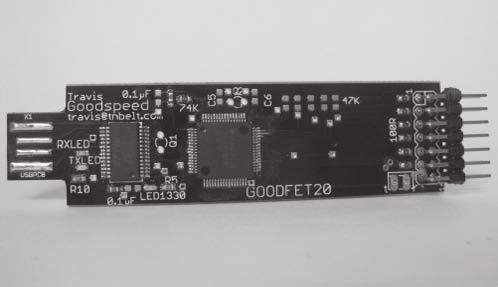
\includegraphics[scale=0.35]{./img/goodFet.jpeg}
}
Atak taki mógłby przebiegać w następujący sposób:
\begin{enumerate}
	\item Atakujący odkrywa fizyczne położenie węzłów sieci
	\item Atakujący znajduje Trust Center
	\item Za pomocą GoodFET Napastnik zyskuje dostęp do wszystkich kluczy sieciowych
\end{enumerate} 
Ponieważ dla pewnej rodziny popularnych chipów np firmy \textit{Texas Instruments} klucze są przetrzymywane w urządzeniu w postaci nie zaszyfrowanej, oraz w miejscu w pamięci dobrze opisanym w dokumentacji technicznej, ataku tego może dokonać prawie każdy wyposarzony w framework KillerBee oraz narzędzie GoodFET. \\

\par
\tab \textbf{Sniffing pakietów} \\
Ponieważ duża część dostępnych nadajników ZigBee nie wspiera domyślnie (lub czasem całkowicie) szyfrowanego połączenia, Atakujący może z łatwością w takich sieciach przechwycić cały ruch sieciowy. Szyfrowanie w sieciach ZigBee maskuje treść danych natomiast nie ukrywa MAC adresu oraz PAN ID, ten fakt w połączeniu z możliwością fizycznej lokalizacji odbiorników dostarcza dodatkowych możliwości ataku na sieć.\\
W przypadku sieci pracujących w trybie SSM (Standard Security Mode), w momencie przyłączenia nowego węzła do sieci po autentykacji, klucz sieciowy jest wysyłany do urządzenia w postaci nie zaszyfrowanej, a następnie za jego pomocą jest wymieniany \textit{Link Key} (LK jest wysyłany w postaci zaszyfrowanej za pomocą Network Key).\\ 
Powyższy scenariusz umożliwia podsłuchującemu napastnikowi który dołączy do sieci na przechwytywanie kluczy do innych nowych węzłów. Co więcej w momencie kiedy tworzona jest cała sieć a napastnik podsłuchuje komunikację jest w stanie poznać Network Key bez konieczności dołączania do sieci, wystarczy że podsłucha pierwszą wymianę klucza sieciowego, aby tego dokonać Atakujący może namierzyć fizycznie Koordynatora oraz kanał częstotliwości na którym działa sieć po czym po prostu zresetować zasilanie Koordynatora w efekcie czego sieć będzie tworzona od nowa, a napastnik podsłucha wymiany wszystkich kluczy. \\
Problem pasywnego podsłuchiwania rozwiązuje tryb HSM (High security mode) w którym to żadne klucze nie są wymieniane w postaci jawnej a zamiast tego są fabrycznie zapisywane w pamięci urządzeń. To rozwiązanie ma swoje wady jeśli chodzi o elastyczność takiego rozwiązania (np w razie ewentualnej awarii któregoś z urządzeń) ale w zamian za to dostarcza bezpieczne rozwiązanie komunikacyjne. \\

\par
\tab \textbf{Wstrzykiwanie pakietów} \\
Koncept ataku jest bardzo prosty: obserwacja pakietów oraz retransmisja wybranych pakietów (w przypadku sieci zaszyfrowanych) lub w przypadku znajomości kluczy albo sieci jawnych proste tworzewnie własnych pakietów. \\
Sam standard ZigBee zakłada niepodatność protokołu na ataki typu \textit{Reply Attacks} jednakże Autor do tej pory nie spotkał się z implementacją stosu ZigBee który by był odporny na te ataki. Np. dostawca dużego procenta chipów do ZigBee \textit{Texas Instrument} dostarcza stos do swoich układów który jest podatny na atak wstrzykiwania tego samego pakietu. \\
Wyobraźmy sobie taki scenariusz ataku:
\begin{enumerate}
	\item Napastnik poprzez znajomość fizycznego położenia węzłów sieci identyfikuje je z MAC adresami
	\item Atakujący podsłuchuje sieć i wywołuje pewne zdarzenia np. stymuluje sensory lub korzysta z dostępnych włączników/przełączników.
	\item Przy dużej próbie jest w stanie powiązać poszczególne pakiety ze zdarzeniami fizycznymi czy impulsami.
	\item Posiadając mapowanie pakiet-zdarzenie Napastnik może sterować siecią i wywoływać zdarzenia które podsłuchał. Dotyczy to zarówno szyfrowanych sieci (HSM, SSM) jak i jawnych.
\end{enumerate}  

\par
\tab \textbf{Przechwytywanie transportu klucza} \\
Standard ZigBee wprowadza dodatkowe mechanizmy służące rozprowadzaniu kluczy, takie jak prekonfiguracja (ustawienie klucza na urządzeniu podczas procesu wytwarzania) negocjacja klucza (Protokół \textit{SKKE - Symmetric-Key Key Establishment}). Prekonfiguracja jest wymagana w trybie \textit{HSM} zapewnia ono wysokie bezpieczeństwo ale również bardzo trudną późniejszą rekonfiguracje każdego z urządzeń w sieci.\\
Natomiast mechanizm SKKE wprowadzony w versji ZigBee-Pro umożliwia prostą i elastyczną rekonfigurację w oparciu o Trust Center. Niestety SKKE jest niewystarczającym mechanizmem zabezpieczającym i może być łatwo złamany albo podsłuchany tak jak to zostało wspomniane wcześniej. Z tego powodu we wszystkich zastosowaniach w których wymagane jest wysokie bezpieczeństwo należy wystrzegać się mechanizmów opartych o kryptografię symetryczną takich jak SKKE ponieważ w nich najczęściej występuje dystrybucja kluczy lub części klucza umożliwiająca atakującemu na złamanie klucza sesji (lub jego podsłuchanie).



	\subsection{Podsumowanie i wnioski}

\par
\tab Dzięki użyciu modelu CIA zademonstrowanemu na początku rozdziału można odnieść system rzeczywisty do teoretycznego modelu w każdym z trzech wymiarów (Poufność, Integralność i Dostępność).

\subsection{Integralność - Integrity}
\par
\tab Kwestie związane z Integralnością danych otrzymywanych przez oba protokoły: \textit{ZigBee i Bluetooth Low Energy} nie były empirycznie sprawdzane ponieważ obydwie specyfikacje (w przypadku ZigBee - 802.15.4 dla BLE 802.15.1) zawierają stosowne wymogi oraz mechanizmy dbające o integralność przesyłanych danych zarówno na poziomie warstwy fizycznej jak i programowej (stos protokołu). Z tego powodu korzystając z któregoś z tych interfejsów komunikacyjnych integralność danych dostajemy nie jako "z pudełka".


\subsection{Dostępność - Availability}
\par
\tab Dostępność danych została zbadana pod kontem niezawodności oraz szybkości odpowiedzi w czasie. Oba protokoły: \textit{ZigBee i Bluetooth Low Energy} spełniają wymagania dostępności oraz gwarantują pewną odpowiedz w z góry ustalonym czasie.
Dzięki temu konstruując system WSN lub RT można sobie założyć kilku milisekundowe opóźnienie wynikające z wymaganego czasu na przeprowadzenie transmisji RF oraz obsłużeniu przez system po obu stronach zdarzenia.

\subsection{Poufność - Confidentiality}
\par
\tab Poufność danych oraz kwestie z nieautoryzowanym dostępem do danych zostały przeanalizowane w oparciu o najnowsze badania instytutów związanych z bezpieczeństwem elektronicznym oraz niezależnych konsultantów. \\
W momencie kiedy potrzebujemy bezpiecznego systemu w którym dane przesyłane między urządzeniami mają być tajne oraz ich pochodzenie musi być niepodważalne, należy wyeliminować rozwiązania oparte o protokół BLE ponieważ na dzień dzisiejszy nie zapewnia on żadnego bezpieczeństwa przed przygotowanym napastnikiem. Również przy sieciach ZigBee należy odrzucić rozwiązania takie jak SSM \textit{(Standard Secuirty Mode)} czy tym bardziej nie szyfrowaną konfigurację sieci. ZigBee w trybie HSE \textit{(High Secuirty Mode)} wydaje się być dobrym wyborem ponieważ zapewnia ono bezpieczeństwo przed podsłuchiwaniem, czy przechwytywaniem klucza. Niestety tryb HSE posiada jedną krytyczną lukę a mianowicie podatność na atak wstrzykiwania pakietów przed którym trzeba się zabezpieczyć w wyższych warstwach protokołu a mianowicie w warstwie aplikacji. \\

\subsection{Zabezpieczenie ZigBee HSE przed Atakiem \textit{Packet Injection} }
\par
\tab Aby zabezpieczyć się przed atakiem typu \textit{Packet Injection} który był opisany w ostatniej sekcji rozdziału 4.3 należy skorzystać z rozwiązania znanego z systemów zabezpieczeń samochodowyh firmy MicroChip \textit{KeeLoq}. KeyLoq jest protokołem opierającym się o kryptografię symetryczną stosowany w centralnych zamkach, jest on nie podatny na ataki typu \textit{Replay Attack} w których to napastnik podsłuchałby transmisji między kluczykiem RF a samochodem i w przyszłości reużyłby tej transmisji w celu odbezpieczenia samochodu. \\
Idea zabezpieczenia jest bardzo prosta: Każdy z wysyłanych pakietów ma swój numer który jest zwiększany o 1 przy każdej transmisji i tworzy on chronologiczną zależność między pakietami. Numer ten jest szyfrowany w ramce danych dla tego atakujący nie jest w stanie go odszyfrować bez znajomości hasła. Numer ten jest na początku równy zeru i przy każdej transmisji odbiornik sprawdza czy otrzymany pakiet ma numer większy czy mniejszy bądz równy ostatniemu pakietowi. Jeśli ten numer jest większy pakiet jest normalnie przetwarzany natomiast jeśli nie pakiet zostaje ignorowany. \\
Dodatkowo aby zabezpieczyć się przed "przekręceniem licznika" do numeru pakietu należy dodać losowy znak który również będzie ignorowany ale sprawi on że nigdy nie wystąpi sytuacja w której powstaną dwa identyczne pakiety i uniemożliwi to atakującemu na wstrzyknięcie pakietu. \\
W celu poznania większej liczby szczegółów na temat obrony KeyLoq przed  \textit{Replay attack} należy skorzystać ze źródeł podanych w bibliografi. \\

\mbox{}\\
\begin{tabular}{ |p{3cm}||p{3cm}|p{3cm}|p{3cm}|  }
 \hline
 \multicolumn{4}{|c|}{Porównanie zgodnie z modelem CIA ZigBee i BLE} \\
 \hline
 Wymiar & Integrity & Availability & Confidentiality\\
 \hline
 Zigbee  & v  & v 	&   v*\\
 BLE 	 & v   & v  & x\\
 \hline
\end{tabular}
* {\small W trybie HSM i z programowym zabezpieczeniem przed packet injections. \par}  
\mbox{}\\

\subsection{Poodsumowanie}
\par
\tab Po przeanalizowaniu systemu w wymiarach: Integralności i Dostępności zarówno BLE jak i ZigBee prezentują się bardzo dobrze i nie ma między nimi dużych różnic. Największą możliwą różnicą w zastosowaniu jest możliwość integracji BLE z zewnętrznymi komercyjnymi urządzeniami dostępnymi na rynku takimi jak smartphony czy tablety, ponieważ ZigBee jako przemysłowy protokół komunikacji nie znajduje się w konsumenckich urządzeniach elektronicznych. Z drugiej natomiast strony Bluetooth Low Energy nie umożliwia stworzenia architektury sieciowej o wielu urządzeniach podłączonych do sieci. \\
Porównując ZigBee i BLE w wymiarze bezpieczeństwa mamy tutaj znaczną przewagę protokołu ZigBee wobec protokołu Bluetooth Low Energy który sam z siebie nie zapewnia praktycznie żadnego bezpieczeństwa. Dobierając fizyczne układy do projektu kiedy decydujemy się na ZigBee należy również pamiętać że nie wszystkie dostępne na rynku moduły RF mogą pracować w trybie HSM, z tego powodu dobór odpowiedniego modułu może się wiązać z dodatkowymi kosztami które również trzeba uwzględnić.\\

Dobierając protokół komunikacyjny trzeba na pierwszym miejscu przeanalizować jego warunki pracy, architekturę rozwiązania oraz współpracę z innymi urządzeniami, systemami. Jeśli bierzemy pod uwagę również kwestię bezpieczeństwa to zawsze zaleca się z korzystania z standardowych rozwiązań bezpieczeństwa dostarczanych przez protokół komunikacyjny (tzw: \textit{Out Of The Box}) z którego się korzysta, w tym wypadku ZigBee okazuje się właściwym wyborem. Jednak czasem jeśli kluczową kwestią jest integracja z zewnętrznymi urządzeniami takimi jak telefony i tablety, BLE staje się bardziej pożądanym wyborem. W takim przypadku gdy bezpieczeństwo jest porządaną cechą należy zastanowić się nad innymi zastosowaniami dostępnymi na rynku takimi jak Wifi lub skorzystanie z gotowych bibliotek kryptograficznych dostępnych na rynku. Często jednak wprowadzenie zewnętrznej kryptografii na poziomie aplikacji bywa kłopotliwe, kosztowne czasowo oraz pochłaniające dużą część zasobów mikrokontrolera. Fakt ten może skłonić konstruktora do ponownego przemyślenia innych rozwiązań bezprzewodowych opartych o internet: Wifi, 6LoWPAN. 

\clearpage

\clearpage

\section{Bibliografia}

//Zigbee: 

Shahin Farahani : ZigBee Wireless Networks and Transceivers \\ 

Robert Faludi : Building Wireless Sensor Networks \\

ZigBee Alliance : ZigBee Specification Document 053474r17 \\

//BLE:

Robin Heydon : Bluetooth Low Energy: The Developer's Handbook \\

Kevin Townsend, Carles Cufí, Akiba, Robert Davidson : Getting Started with Bluetooth Low Energy \\

//General:

Johnny Cache, Joshuda Wright and Vincent Liu : Wireless Hacking Exposed \\

James W. Grenning : Test-Driven Development for Embedded C \\

Elecia White : Making Embedded Systems: Design Patterns for Great Software \\
	
David Kleidermacher, Mike Kleidermacher : Embedded Systems Security: Practical Methods for Safe and Secure Software and Systems Development \\

Marcin Bis : Materiały do szkoleń "Systemy czasu rzeczywistego" \\

John Viega and Matt Messier : Secure Programming Cookbook for C and C++ \\

Joshuda Wright : Prezentacja "KillerBee: Practical ZigBee Exploitation Framework" \\

Dominic Spill Andrea Bittau : "BlueSniff: Eve meets Alice and Bluetooth" \\

Tomáš Rosa : "Bypassing Passkey Authentication in Bluetooth Low Energy" \\

Mike Ryan (and iSEC Partners) : "Bluetooth: With Low Energy comes Low Security" \\

Bjorn Stelte and Gabi Dreo Rodosek : "Thwarting Attacks on ZigBee – Removal of the KillerBee Stinger" \\

KeeLoq : http://en.wikipedia.org/wiki/KeeLoq
\clearpage

\end{CJK*}	
\end{document}